\documentclass[12pt,italian]{article}
\usepackage[T1]{fontenc}
\usepackage{babel}
\usepackage[utf8]{inputenc}
\usepackage{enumitem}
\usepackage{subfiles}
\usepackage{multirow}
\usepackage{color}
\usepackage{titlesec}
\usepackage{longtable}
\usepackage{xcolor,colortbl}
\usepackage[hidelinks]{hyperref}
\usepackage{graphicx}
\usepackage{adjustbox}
\usepackage{amsmath}
\usepackage{mdframed}
\usepackage{listings}
\usepackage{minted}
\usepackage{subfigure}
\usepackage{changepage}

\usepackage[a4paper,right=25mm,top=25mm,bottom=25mm, left=25mm]{geometry}
\usepackage{afterpage}
\usepackage{array,ragged2e}
\usepackage{booktabs}


\graphicspath{
  {./immagini/}
}

\definecolor{LightGray}{gray}{0.9}

\definecolor{codegreen}{rgb}{0,0.6,0}
\definecolor{codegray}{rgb}{0.5,0.5,0.5}
\definecolor{codepurple}{rgb}{0.58,0,0.82}
\definecolor{backcolour}{rgb}{0.95,0.95,0.92}

\newcolumntype{P}[1]{>{\RaggedRight\arraybackslash}p{#1}}
\renewcommand{\baselinestretch}{1.5} 

\newlist{tabitem}{itemize}{1}
\setlist[tabitem]{nosep,
                  topsep     = 0pt,
                  partopsep  = 0pt,
                  leftmargin = *,
                  label      = \textbullet,
                  before = \vspace{-1\baselineskip},
                  after = \vspace{-0.5\baselineskip}}

\hypersetup{
    linktoc=all,
    pdfpagemode=FullScreen,
}
\definecolor{Gray}{gray}{0.85}
\definecolor{LightCyan}{rgb}{0.88,1,1}


\newcommand{\mycomment}[1]{}

\mycomment{}

\begin{document}


\begin{titlepage}
    
\pagestyle{empty}
\newgeometry{
    left=20mm,
    right=20mm,
    top=20mm,
    bottom=20mm
}


\begin{center}

% marchio di ateneo

\includegraphics[width=6.5cm,height=4.7cm]{marchio-di-ateneo_gs.png}

\vspace{10mm}

% \large is 12pt
{\normalsize{\bf{DIPARTIMENTO DI INFORMATICA - SCIENZA e INGEGNERIA}}} 

\vspace{5mm}

{\large{\bf{CORSO DI LAUREA MAGISTRALE IN INGEGNERIA INFORMATICA}}}

\vspace{23mm}

{\LARGE{\bf Analisi, Progettazione e Distribuzione in Cloud di applicativo multipiattaforma}}\\
\vspace{3mm}
{\LARGE{\bf per l'organizzazione di eventi condivisi e la condivisione multimediale automatica in tempo reale}}\\
\vspace{3mm}
%{\Huge{\bf }}\\
\vspace{3mm}

\end{center}

\vspace{32mm}

\begin{minipage}[t]{0.40\textwidth}
{\Large{\bf Relatore: \\ Chiar.mo Prof.\\ Michele Colajanni}}

\vspace{3mm}

{\Large{\bf }}
\end{minipage}
\hfill
\begin{minipage}[t]{0.40\textwidth}\raggedleft
{\Large{\bf Presentata da: \\ Giacomo Romanini}}
\end{minipage}

\vspace{10mm}

\rule[0.5cm]{15.8cm}{0.6mm}

\begin{center}
{\large{\bf Sessione Marzo 2025 \\}}
{\large{\bf Anno Accademico 2024/2025\\}}
\end{center}

\end{titlepage}

\restoregeometry



\section*{Abstract}


Lo sviluppo di un applicativo multipiattaforma diretto all’organizzazione di eventi condivisi, 
caratterizzato in particolare dalla condivisione multimediale in tempo reale, richiede opportune capacità di scalabilità, 
atte a garantire una risposta efficace anche con alti volumi di richieste, offrendo prestazioni ottimali. 
Le tecnologie cloud, con la loro disponibilità pressoché illimitata di risorse e alla completa e continua garanzia  di manutenzione, 
offrono l'architettura ideale per il supporto di simili progetti. \\
Tuttavia, l'integrazione tra la logica applicativa ed i molteplici servizi cloud, insieme alla gestione delle loro interazioni reciproche, 
comporta sfide specifiche, in particolare legate all'ottimizzazione di tutte le risorse. 
L’individuazione e la selezione delle soluzioni tecnologiche più adatte per ogni obiettivo
e l'adozione delle migliori pratiche progettuali devono procedere parallelamente con lo sviluppo del codice, al fine di sfruttare efficacemente le potenzialità offerte. \\
In tale prospettiva, questa tesi illustra le scelte progettuali e implementative adottate nello sviluppo dell'applicativo in questione, 
evidenziando l’impatto dell'integrazione delle risorse cloud sul risultato finale.
\clearpage
\pagenumbering{roman}
\tableofcontents
\clearpage
\pagenumbering{arabic}


\section*{Introduzione}
\addcontentsline{toc}{section}{Introduzione}


In un contesto sempre più connesso, la crescente quantità di contatti, la rapidità delle comunicazioni e l'accesso universale alle informazioni rendono la creazione, l'organizzazione e la partecipazione ad eventi estremamente facile, ma al contempo generano un ambiente frenetico e spesso dispersivo.\\
Risulta infatti difficile seguire tutte le opportunità a cui si potrebbe partecipare, considerando le numerose occasioni che si presentano quotidianamente, rischiando di ricordarsene solo successivamente, una volta passate. Basti pensare, ad esempio, alle riunioni di lavoro, alle serate con amici, agli appuntamenti informali per un caffè, ma anche a eventi più strutturati come fiere, convention aziendali, concerti, partite sportive o mostre di artisti che visitano occasionalmente la città.\\
Questi eventi possono sovrapporsi, causando dimenticanze o conflitti di pianificazione, con il rischio di delusione o frustrazione. Quando si è invitati a un evento, può capitare di essere già impegnati, o di trovarsi in attesa di una conferma da parte di altri contatti. In questi casi, la gestione degli impegni diventa complessa: spesso si conferma la partecipazione senza considerare possibili sovrapposizioni, o dimenticandosi, per poi dover scegliere e disdire all'ultimo momento. \\
D’altra parte, anche quando si desidera proporre un evento, la ricerca di un'attività interessante può diventare un compito arduo, con la necessità di consultare numerosi profili social di locali e attività, senza avere inoltre la certezza che gli altri siano disponibili.\\
Tali problemi si acuiscono ulteriormente quando si tratta di organizzare eventi di gruppo, dove bisogna allineare gli impegni di più persone. \\
In questo contesto, emergono la necessità e l'opportunità di sviluppare uno strumento che semplifichi la proposta e la gestione degli eventi, separando il momento della proposta da quello della conferma di partecipazione. In tal modo, gli utenti possono valutare la disponibilità degli altri prima di impegnarsi definitivamente, facilitando l'invito e la partecipazione.\\ 
\clearpage
In risposta a tali richieste è nata Wyd, un'applicazione che permette ai clienti di organizzare i propri impegni, siano essi confermati oppure proposti. Essa permette anche di rendere più intuitiva la ricerca di eventi attraverso la creazione di uno spazio virtuale centralizzato dove gli utenti possano pubblicare e consultare tutti gli eventi disponibili, diminuendo l’eventualità di perderne qualcuno. 
La funzionalità chiave di questo progetto si fonda sull'idea di affiancare alla tradizionale agenda degli impegni certi un calendario separato, che mostri tutti gli eventi a cui si potrebbe partecipare. Una volta confermata la partecipazione a un evento, questo verrà spostato automaticamente nell'agenda personale dell'utente.
Gli eventi creati potranno essere condivisi con persone o gruppi, permettendo di visualizzare le conferme di partecipazione. 
Inoltre, considerando l'importanza della condivisione di contenuti multimediali, questo progetto prevede la possibilità di condividere foto e video con tutti i partecipanti all'evento, attraverso la generazione di link per applicazioni esterne o grazie all'ausilio di gruppi di profili. Al termine dell’evento,
l'applicazione carica automaticamente le foto scattate durante l'evento,
per allegarle a seguito della conferma dell'utente.\\
\\
Come anticipato, la realizzazione di un progetto come Wyd implica la risoluzione e la gestione di diverse problematiche tecniche. 
In primo luogo, garantire la persistenza dell'agenda dell'utente, che deve essere aggiornata e mantenuta in modo affidabile e coerente, tale da permettere per un uso distribuito del servizio. 
Inoltre, la funzionalità di condivisione degli eventi richiede l'aggiornamento in tempo reale di tutti gli utenti coinvolti, al fine di rimanere sempre aggiornati. 
Infine, il caricamento e il salvataggio delle foto introduce la necessità di gestire richieste di archiviazione di dimensioni significative.
In questa prospettiva, risulta fondamentale esplorare il procedimento di analisi e progettazione che ha portato allo sviluppo di un applicativo multipiattaforma efficace, affidabile e scalabile, in grado di soddisfare le esigenze degli utenti nell’ambito dell'organizzazione di eventi condivisi e della condivisione multimediale automatica in tempo reale.
Seguendo l’esame dei requisiti necessari, l’analisi dello sviluppo del progetto affronterà in una prima parte le scelte infrastrutturali che hanno portato a definire la struttura centrale dell’applicazione, spiegando brevemente i requisiti e le soluzioni trovate. 
Successivamente si osserverà lo studio effettuato per gestire la memoria, in quanto fattore che più incide sulle prestazioni. Particolare attenzione è stata dedicata, infatti, a determinare le tecnologie e i metodi che meglio corrispondono alle esigenze derivate dal salvataggio e dall’interazione logica degli elementi.
Infine, per permettere la gestione delle immagini, che introducono problematiche impattanti sia sulle dimensioni delle richieste sia sull'integrazione con la persistenza, una terza parte si concentrerà sulle scelte implementative adottate per l’inserimento delle funzionalità.


\clearpage

-\section{Struttura centrale}

Durante lo sviluppo del prodotto, in fase di progettazione, che ha lo scopo di identificare le caratteristiche funzionali e comportamentali dell’applicazione, vengono evidenziate le parti principali del programma con le relative funzioni assolte.\\
\\
Le prime scelte della fase successiva, l’implementazione, riguardano l’architettura e le tecnologie del sistema. La loro relazione specifica il comportamento dei componenti e determina le modalità con cui si interfacciano tra loro.\\
\\
L’abilità di trovare le migliori soluzioni che più si adattano alla risoluzione delle esigenze rispettando i requisiti espressi in fase di progettazione comporta fin da subito uno sviluppo corretto ed efficiente.  \\
\\

\begin{figure}[h!]
    \centering
    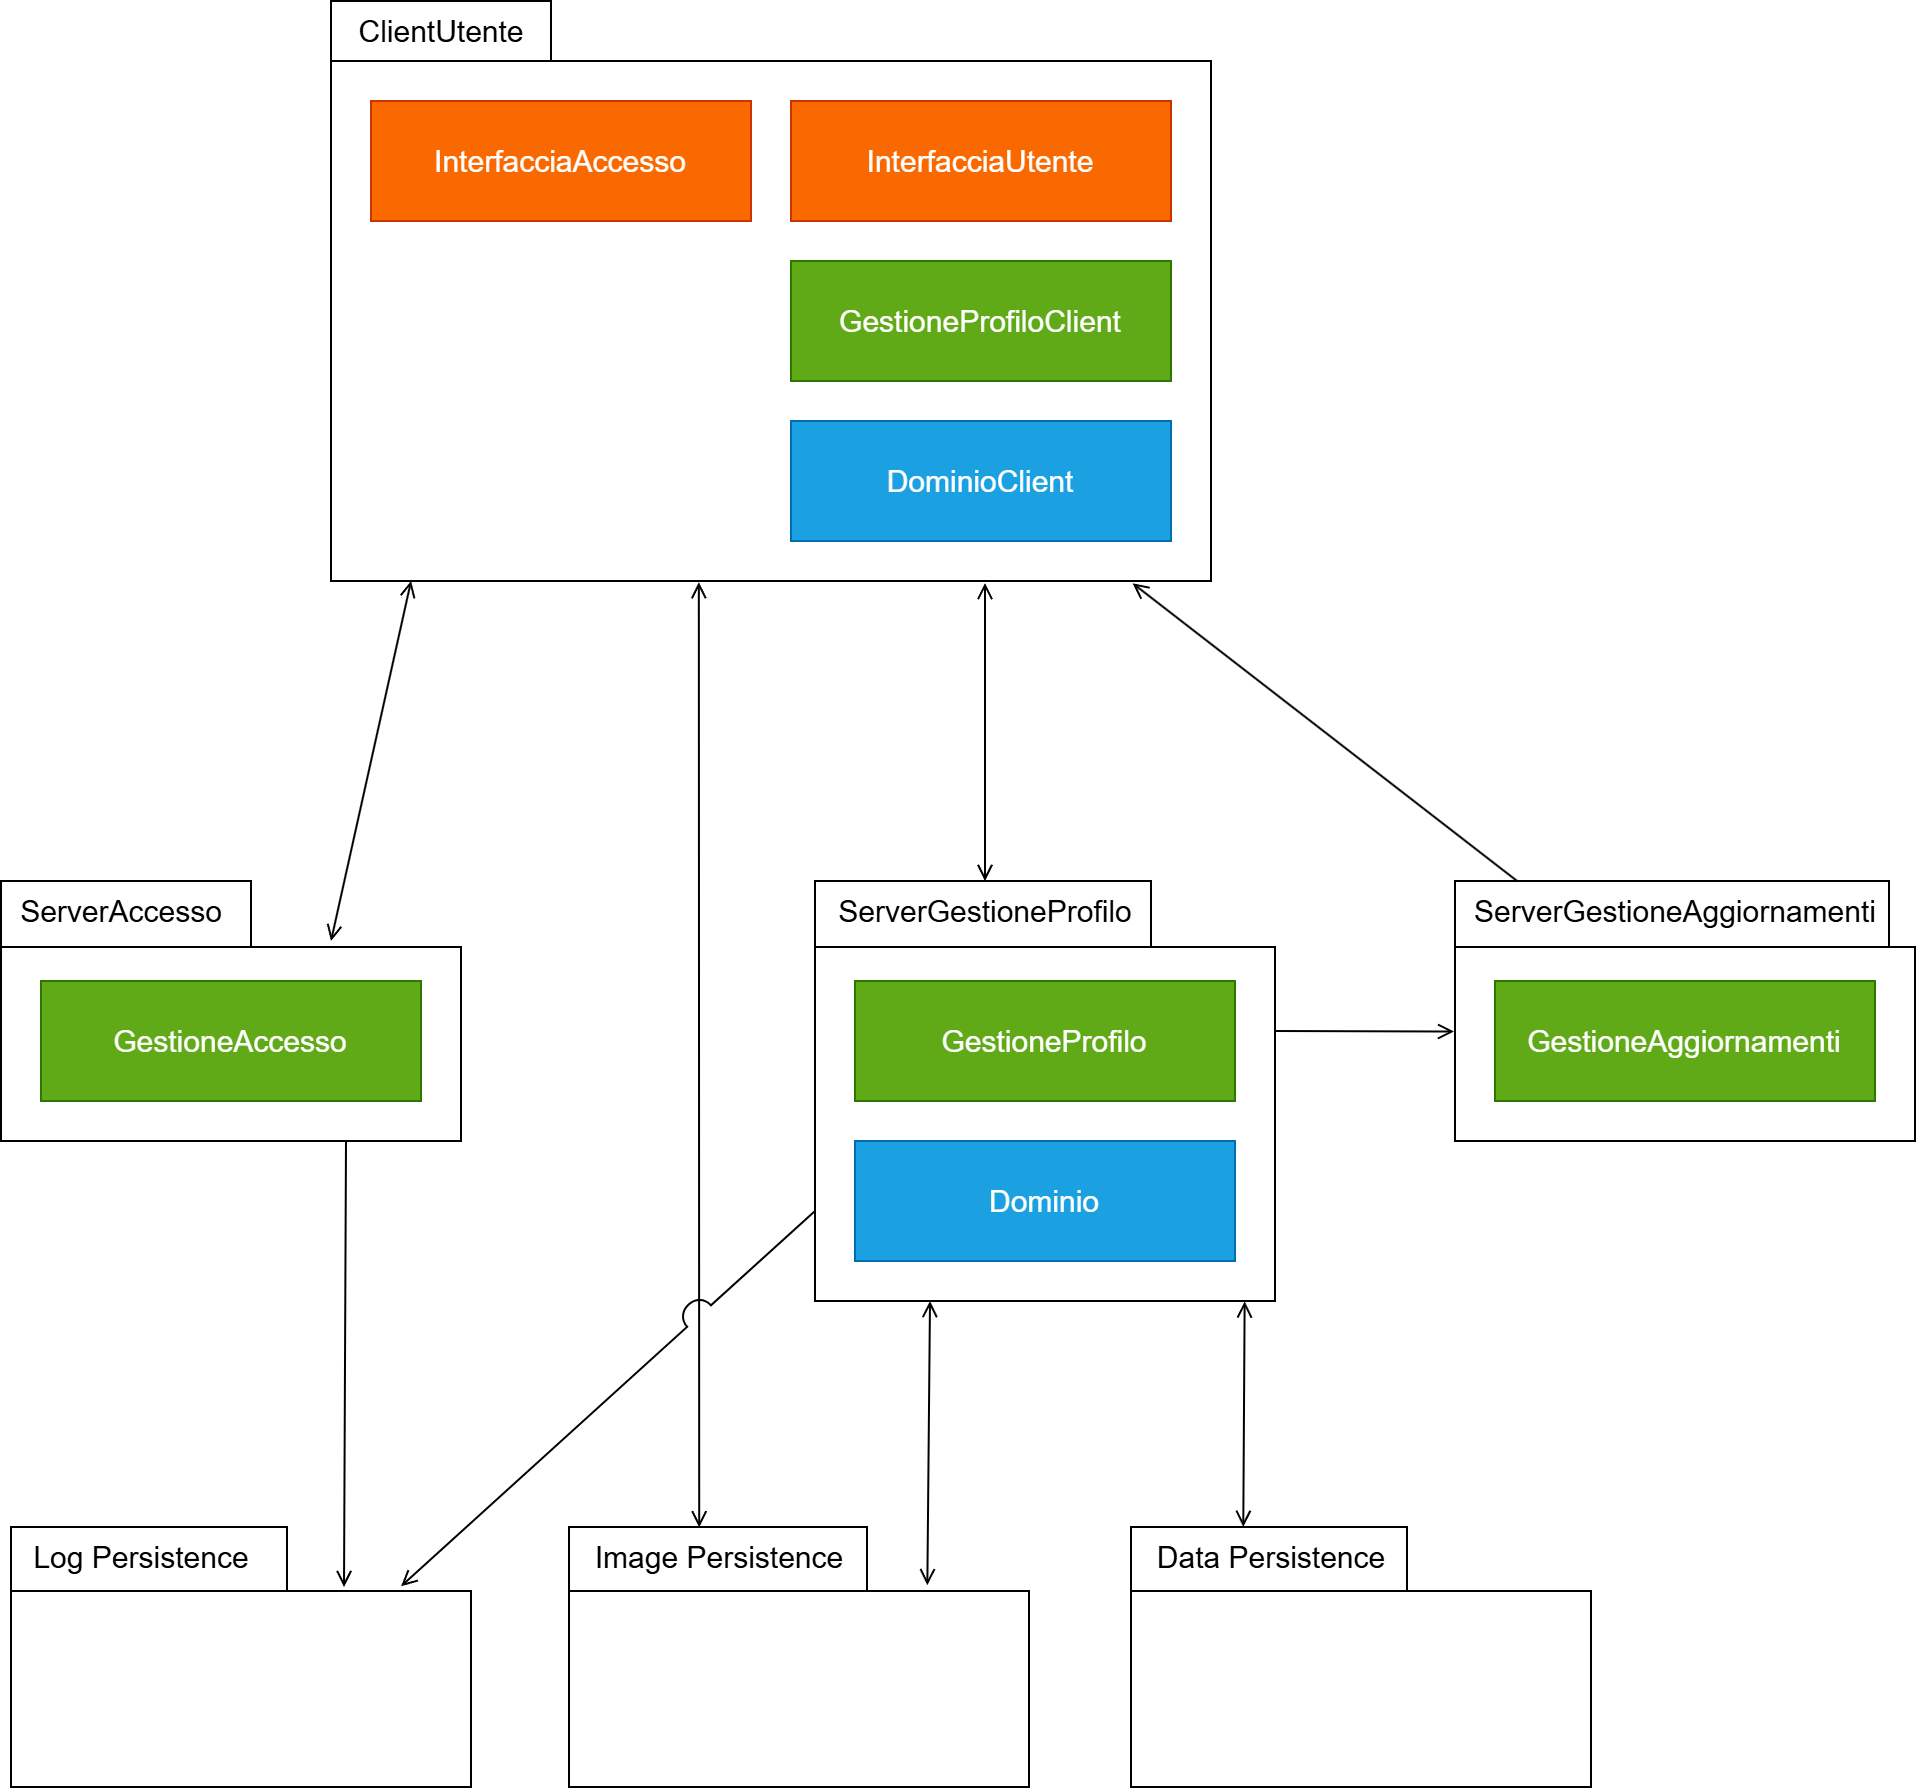
\includegraphics[width=\textwidth]{ProgettoDiagrammaPackage.png}
    \caption{Struttura e responsabilità delle parti del progetto}
\end{figure}
Sebbene per alcune parti le decisioni possano risultare semplici o intercambiabili, altre possono dover richiedere ulteriori analisi. Risulta conveniente sviluppare prima i componenti di cui sono ben definiti i requisiti ed è presente una soluzione chiara che risponde alle esigenze specifiche. L’identificazione, anche parziale, di una struttura iniziale determina ulteriori requisiti di integrazione che facilitano l’individuazione delle restanti soluzioni necessarie.

\clearpage
\subsection{Sviluppo del Client}

L’utilizzo delle applicazioni per la gestione degli eventi può essere suddiviso in due fasi distinte, ciascuna con specifiche esigenze funzionali. 
La prima fase riguarda infatti la pianificazione a lungo termine e l’organizzazione degli impegni. In questo tempo l’utente decide come distribuire il proprio tempo, pianificando attività e appuntamenti, e strutturando il proprio calendario nel modo più efficiente per le proprie necessità. 
La seconda fase riguarda invece la gestione degli eventi non ancora certi e definiti; ciò include l’invito a un evento, l’eventuale conferma da parte dell’utente, l’identificazione degli impegni a breve termine e l’aggiornamento del loro stato (ad esempio, se l’evento sia ancora confermato, quante persone vi partecipano, se qualcuno ha annullato o se l'evento è già concluso) con la gestione degli eventuali contenuti multimediali successivi all’evento. Queste due fasi implicano un approccio diverso da parte dell’utente, comportando di conseguenza esigenze differenti a cui l’applicazione deve rispondere adeguatamente. 
Per rispondere a tali necessità, è fondamentale che l'applicazione offra un'interfaccia utente versatile, fruibile sia da desktop che da dispositivi mobili. La versione desktop consente una pianificazione a lungo termine, offrendo una visione d'insieme chiara e completa di tutti gli impegni, tale da facilitare la gestione del tempo. D'altra parte, la versione mobile deve permettere una gestione rapida e dinamica degli eventi quotidiani, garantendo che l'utente possa rimanere sempre connesso e aggiornato sugli sviluppi in tempo reale.
Inoltre, considerando che l'applicazione è destinata a un utilizzo diffuso e a un'utenza potenzialmente elevata, è necessario garantire tempi di risposta ridotti e una gestione efficiente delle richieste concorrenti. Ciò implica la progettazione di un sistema in grado di scalare facilmente, per supportare un ampio numero di utenti simultanei senza compromettere le prestazioni.

Al fine di ottenere tutte le prestazioni precedentemente elencate, la scelta è ricaduta sull’adozione del framework di sviluppo Flutter. Diversi fattori motivano tale decisione. 
In primo luogo, l'architettura di Flutter si basa su un motore grafico indipendente dalla piattaforma di esecuzione, il che consente di ottenere elevate prestazioni e garantire un'esperienza utente uniforme su dispositivi diversi. 
In secondo luogo, Flutter adotta un approccio dichiarativo nella progettazione dell'interfaccia grafica, che facilita lo sviluppo di componenti reattivi e scalabili attraverso un codice conciso, facilmente manutenibile.
Un ulteriore vantaggio di Flutter è rappresentato dalla crescente adozione nel settore, dalla solidità della community di sviluppo e dal supporto offerto da Google, che ne assicurano la stabilità, l'efficienza, la sicurezza e la disponibilità di componenti personalizzabili per l'intero ciclo di vita del prodotto. 
Infine, Flutter consente uno sviluppo rapido e interattivo grazie alla sua sintassi intuitiva e al meccanismo di hot reload, che riduce significativamente i tempi di compilazione e facilita il testing in tempo reale.

Tra le altre tecnologie valutate per lo sviluppo dell'interfaccia grafica, vi erano React Native e Xamarin. Tuttavia, entrambe presentano alcune limitazioni: le applicazioni finali sviluppate con React Native tendono ad avere dimensioni più elevate e le prestazioni risultano inferiori, in particolare nella gestione della memoria. Xamarin, pur essendo una valida opzione, presenta una curva di apprendimento più ripida e una comunità di sviluppatori più ridotta rispetto a Flutter, con una conseguente minore disponibilità di componenti e librerie.

Per quanto Flutter consenta di uniformare l'esperienza utente su dispositivi diversi e semplifichi la compilazione per le varie piattaforme, alcune configurazioni rimangono comunque dipendenti dalla tecnologia su cui l'applicazione viene eseguita. Di conseguenza, ciascun eseguibile richiede una manutenzione aggiuntiva, inclusi gli aggiornamenti delle dipendenze specifiche, sia a livello di deployment che di gestione delle versioni.

In una fase iniziale dello sviluppo, nell'ottica di coprire il più ampio mercato possibile con il minor numero di piattaforme, si è deciso di sviluppare una versione fruibile via web e una per dispositivi Android.

 Nell'ambito delle tecnologie Azure, per la  distribuzione del codice web è stato scelto Azure Static Web App, un servizio che permette di ospitare un sito web che non presenta caratteristiche dinamiche, ovvero nel quale la pagina restituita non varia in base all’utente che la richiede. L’applicazione in questione, per scelte progettuali, richiede i dati specifici dell’utente (se non li ha già in una cache locale) solo al server, rendendo l’interfaccia grafica completamente indipendente dall’utente che ne usufruisce.
La robustezza del servizio garantita dalla firma Azure e il suo prezzo ridotto per un uso limitato del servizio sono state ritenute caratteristiche sufficienti per la sua selezione.

Infine, in attesa della pubblicazione dell’applicazione sull’App Store di Android, l’esecutivo è stato reso disponibile tramite Azure Storage Container, un servizio che permette il salvataggio di file di differenti tipologie, allegando un link per il recupero. 

Il codice distribuito sulla web app e l'applicativo salvato sul container verranno aggiornati automaticamente tramite GitHub Actions.
Nella fruizione tramite browser il codice si aggiorna ad ogni accesso, mentre l'applicativo necessita di venire re-installato. Per questa ragione, gli utenti che usano l'applicazione verranno notificati nel momento del caricamento di una nuova versione.

\clearpage
\subsection{Architettura del server principale}
	
L’applicazione necessita della capacità di rispondere a quantità elevate di richieste in breve termine. In altre parole, deve essere scalabile. 
Il servizio Azure che meglio risponde a questa esigenza è Azure Functions. Azure Functions è una risorsa che permette di suddividere il codice in nuclei indipendenti tra loro, creando un ambiente di esecuzione unico per ogni richiesta. Questa caratteristica, unita alla virtualizzazione dell’ambiente di esecuzione fornita dai servizi in cloud, rendono possibile una scalabilità potenzialmente infinita.

La responsabilità dell’indipendenza di ogni funzione e della sua proprietà di essere stateless(ovvero svincolata dal contesto in cui viene eseguita, senza conoscenze dello stato o della sessione), ricade sullo sviluppatore. Ogni funzione assolve un unico compito, seguendo il principio di singola responsabilità. Nel caso in cui una richiesta richieda l’esecuzione di più compiti, Azure Function mette a disposizione la tecnologia Azure Durable Functions. 

Integrata all’interno delle AF, Azure Durable Function permette la creazione di una funzione orchestrator che gestisce l’ordine, lo stato, il tempo di vita e le risposte delle varie funzioni da eseguire per soddisfare la richiesta.
Rimanendo nell’ottica di un ambiente indipendente e scalabile, consente di gestire situazioni in cui l’ordine dei compiti è importante, siano richiesti ulteriori tentativi in caso di fallimento o sia necessaria l’attesa del completamento dei compiti con un tempo di esecuzione elevato.
Per loro natura, le Azure Durable Functions presentano però un tempo di risposta più elevato, a causa della natura stateless e quindi dell’accoppiamento debole con le funzioni che sta eseguendo.  
Grazie a questa tecnologia verranno inizializzate solo le funzioni strettamente necessarie per l’esecuzione di un determinato compito, stanziando al minimo le risorse effettivamente necessarie.

Come linguaggio di programmazione per lo sviluppo delle funzioni è stato utilizzato C\#. L’integrazione con Entity Framework Core permette di mappare direttamente in oggetti i componenti del dominio, semplificando la logica delle relazioni e astraendo le comunicazioni con il database. Grazie all’utilizzo delle proprietà virtuali degli oggetti si rende inoltre possibile il lazy loading, per il quale le richieste al database avvengono solo quando strettamente necessarie. Infine, la consapevolezza che sia l’ambiente di sviluppo di C\#, ovvero il framework .Net, sia la piattaforma Azure sono mantenute dalla stessa azienda, ovvero Microsoft, garantisce il supporto, la stabilità e l’integrazione delle tecnologie.

La piattaforma di sviluppo Visual Studio Code fornisce inoltre la possibilità di collegarsi direttamente ai servizi in cloud tramite estensioni apposite, che rendono l’aggiornamento del codice estremamente semplice e lineare, oltre che immediato.

Azure Function in ambiente .Net permette lo sviluppo in due modalità differenti: in-process worker o isolated worker. Si definisce worker l’applicativo che si occupa di creare le risorse ed eseguire le funzioni in base alle richieste. Nella modalità in-process la funzione eseguirà all’interno dello stesso processo del worker che l’ha creata, riducendo il numero di risorse necessarie ma condividendo l’ambiente di esecuzione. Nel modello isolated ogni funzione viene creata usando un processo unico dedicato, aumentando l’isolamento e quindi riducendo le possibili dipendenze tra le funzioni. Inoltre, il supporto al modello isolated prevede un maggior numero di versioni del framework .Net, che per il modello in-process sono limitate alle sole versioni con supporto a lungo termine. Infine, il supporto per la creazione di un middleware che esegua tra la chiamata e l’esecuzione di una funzione è supportato solo per il modello isolated. 
Per queste ragioni, si è deciso di sviluppare le funzioni usando il modello isolated.

\clearpage
\subsection{Autenticazione}

	La facilità di autenticazione è essenziale per l’esperienza utente. La possibilità di entrare nell’applicazione tramite il proprio authentication provider di fiducia è sicuramente apprezzata, ma allo stesso modo è essenziale offrire la possibilità di creare un account dedicato alla singola applicazione. Il servizio di gestione degli accessi dovrà quindi soddisfare sia l’esigenza di creare account nuovi mantenuti e controllati dall’applicazione, che fornire la possibilità di interagire con i diversi authentication providers.

Azure mette a disposizione il servizio Microsoft Entra ID, all’interno di una famiglia di servizi per l’autenticazione e l’autorizzazione chiamata Microsoft Entra. Per quanto dovrebbe essere in grado rispondere alle funzionalità di cui sopra, la confusione della documentazione e la difficoltà incontrata nell’integrazione con il servizio hanno portato a cercare un’altra soluzione negli ambienti cloud.

La risposta è stata trovata in Firebase Authentication, che garantisce la possibilità di creare account così come di collegarsi ad altri authentication providers. Inoltre, presenta un’interfaccia chiara e offre servizi di integrazione di facile utilizzo sia tramite Flutter che tramite C\#. A livello di costi, il servizio è gratuito sotto i cinquantamila utenti attivi mensilmente.

Tra i requisiti del progetto è richiesto che un account identifichi un solo utente. In fase di creazione del profilo, tuttavia, l’account viene salvato sulla persistenza del server Firebase. 
Si rende necessario, nel momento del primo accesso, che il server, dopo aver controllato l’autenticità della richiesta, crei una copia dell’account, così come il nuovo oggetto utente e il primo profilo relativo.
\begin{figure}[h!]
    \centering
    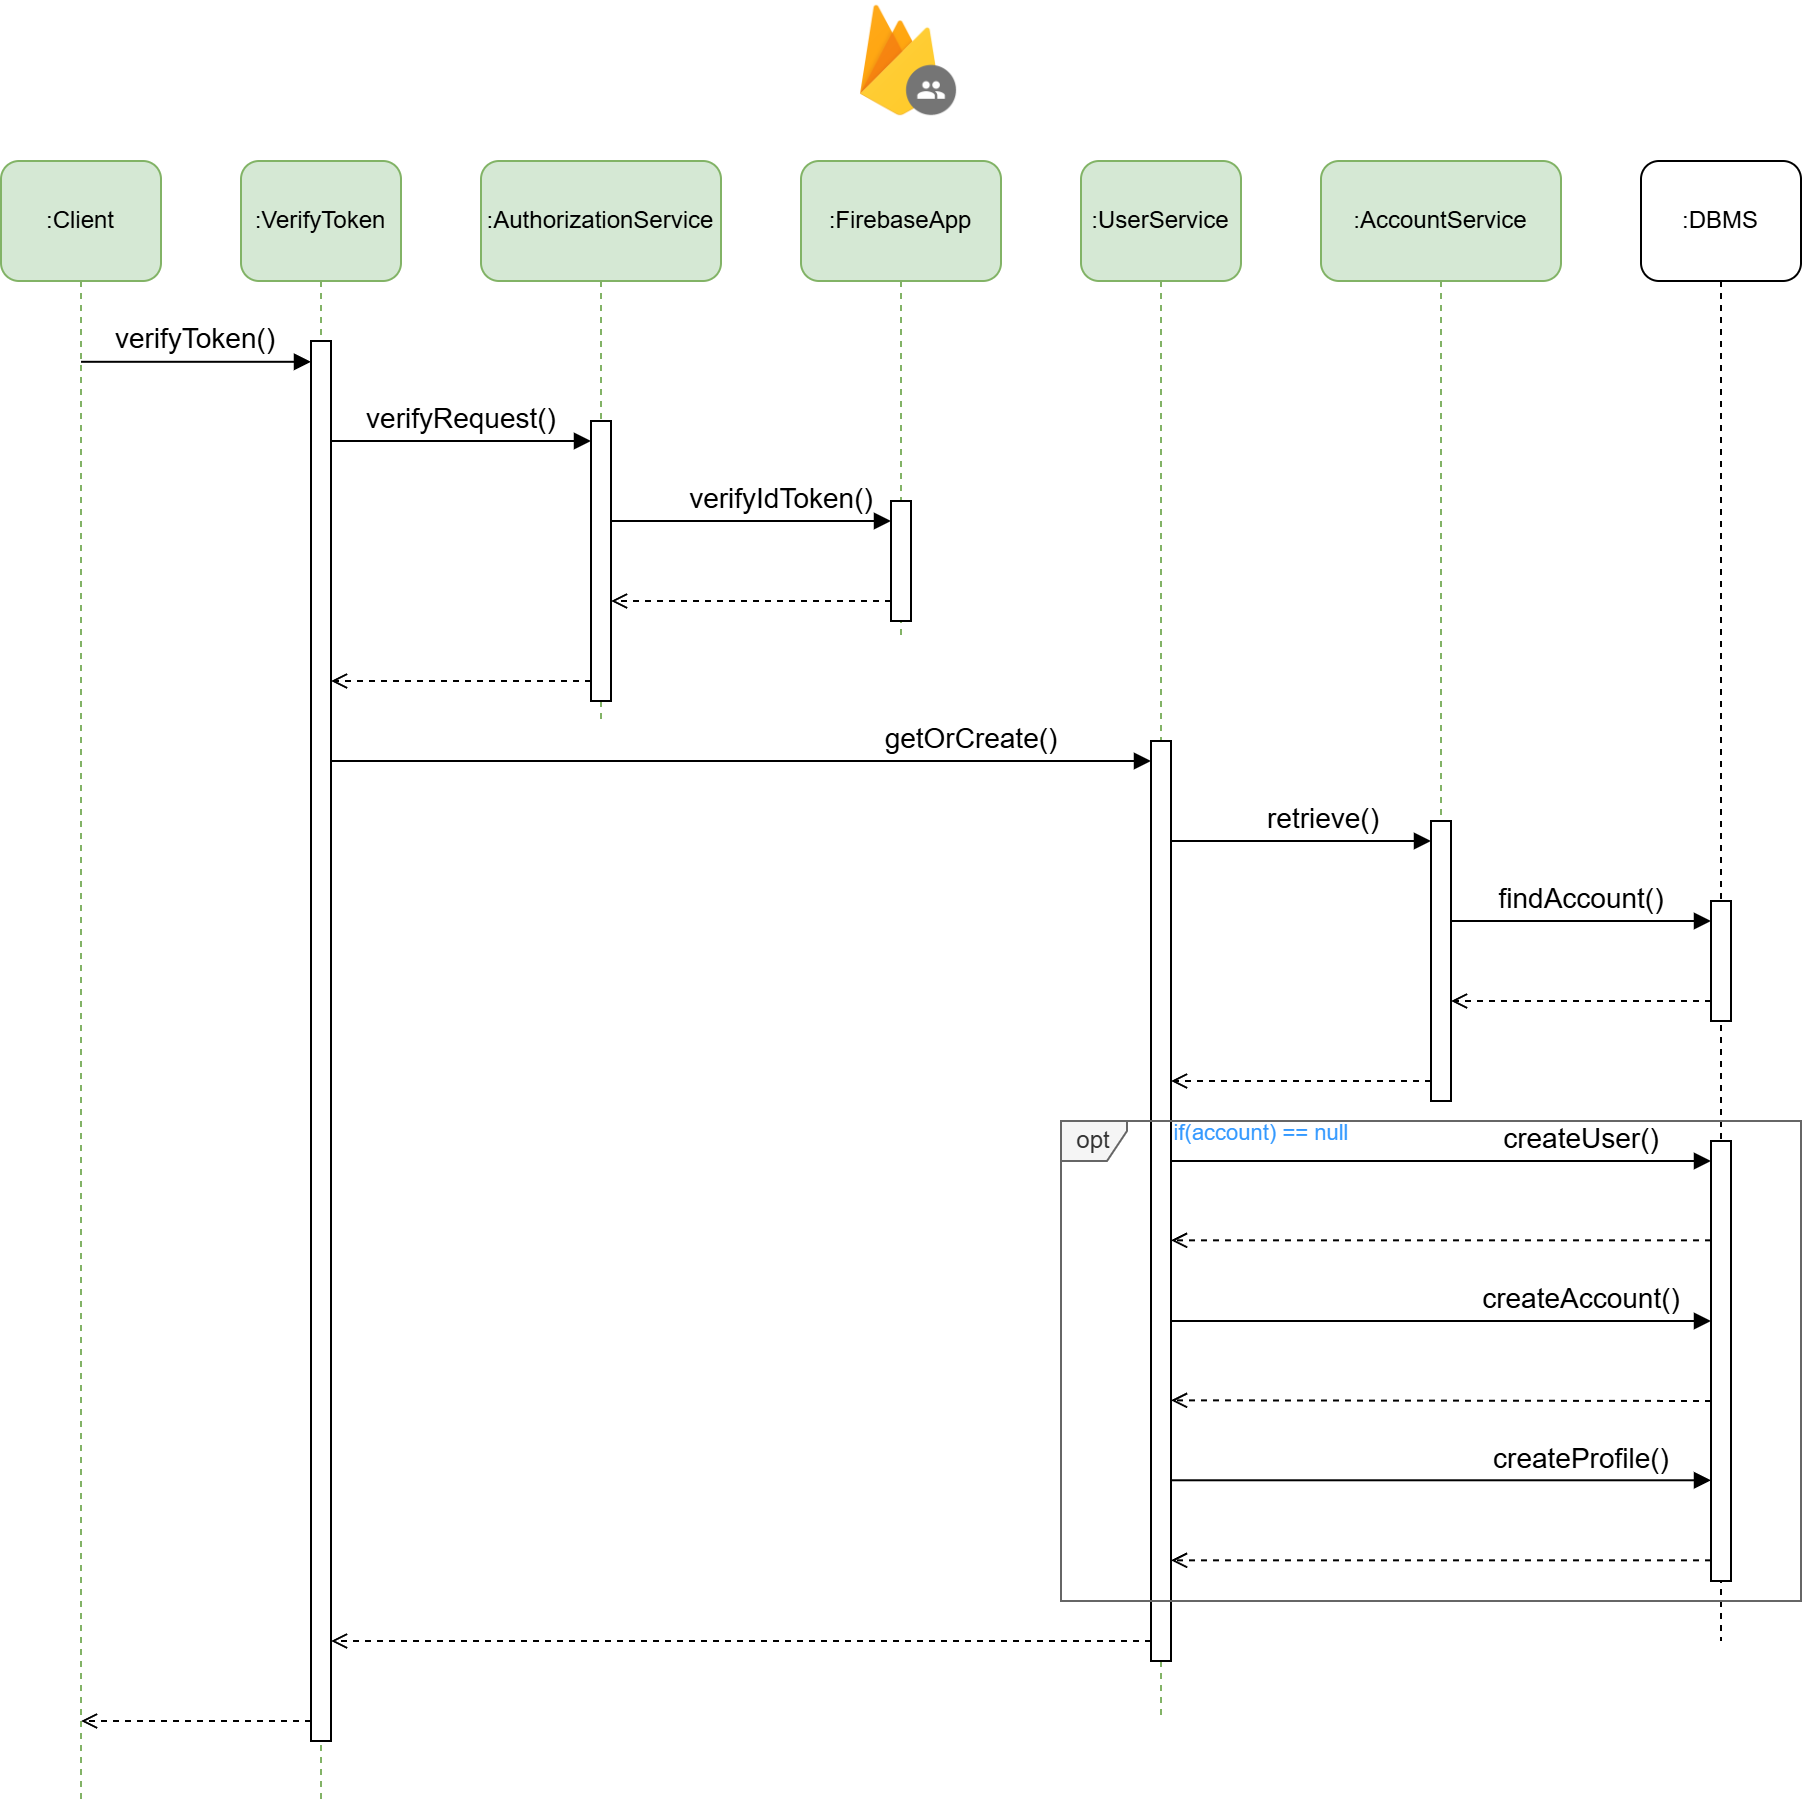
\includegraphics[width=\textwidth]{IIVerifyToken2.png}
    \caption{Diagramma di sequenza per la creazione di un account}
\end{figure}
Ad ogni richiesta in cui sia necessaria l’identificazione, il dispositivo utente aggiungerà alle richieste il token identificativo salvato a seguito dell’autenticazione iniziale. Il server controllerà che il token sia valido, per poi eventualmente proseguire l’esecuzione.


\clearpage
\subsection{Sicurezza}

Il collegamento tra i vari componenti all’interno dell’ambiente Azure richiede l’utilizzo di chiavi e stringhe di connessione. Il salvataggio di tutte le chiavi sensibili è stato affidato al servizio Azure Key Vault, un server che permette la centralizzazione dei dati, cifrando il contenuto e garantendo un controllo maggiore sul loro utilizzo. Quando necessario i servizi, in particolare le Azure Function, contatteranno il Key Vault per l’ottenimento delle chiavi necessarie, riducendo il rischio di un’intercettazione data magari da un errore durante lo sviluppo.

Le comunicazioni tra i vari componenti devono avvenire in sicurezza, garantendo autenticità e confidenzialità. Per questo motivo tutte le comunicazioni tra dispositivi client e i vari servizi utilizzano la tecnologia TLS, che permette di cifrare i messaggi grazie ad uno standard collaudato. In particolare, le comunicazioni tra i client e Azure Function, così come con Firebase Authentication e il server per la persistenza delle immagini, avvengono tramite protocollo HTTPS, mentre le comunicazioni con il server per gli aggiornamenti in tempo reale usano il protocollo WSS.

L’accesso al database è ristretto alle sole risorse Azure, garantendo l’isolamento dall’esterno, che comprometterebbe altrimenti l’affidabilità dei dati.

Infine, l’identificativo di ogni elemento del dominio è nascosto all’utente tramite la creazione di codici hash univoci che permettono comunque l’identificazione dell’oggetto senza rivelare ulteriori informazioni. In particolare, il caricamento delle immagini avviene grazie ad un link univoco dato dalla combinazione degli identificativi dell’evento e dell’immagine. Utilizzando i codici di hash diventa molto complicato il ritrovamento delle immagini senza essere a conoscenza dei codici, che non avendo natura incrementale ma distribuita rende indovinare un link valido.

\clearpage
\subsection{Monitoraggio}

Il monitoraggio del sistema è attuato in due modalità: tramite salvataggio dei log e controllo delle prestazioni del sistema.

Relativamente a Firebase Authentication vengono forniti con il servizio sia le interfacce
per il controllo delle prestazioni che la gestione dei log. Non è quindi richiesta alcuna ulteriore azione.

Per monitorare le Azure Functions sarà invece necessario collegare Azure Application Insights, servizio che provvede a controllare il funzionamento e la risposta del servizio. Una volta unito il servizio, infatti, Azure Application Insight permette la presentazione e l'analisi di numerose metriche, quali il tempo di risposta e il consumo di risorse. Consente inoltre di testare la risposta dell’applicativo simulando diversi scenari e riassumendo il loro comportamento.

La creazione dei log è invece delegata al programmatore, in quanto è necessario integrarli nel codice. Nel momento della creazione, ogni funzione riceve, tramite dependency injection, un servizio Logger che permette la creazione e il salvataggio dei log. Tali log saranno poi consultabili e analizzabili tramite l’interfaccia fornita da Azure Application Insight.

\clearpage
\section{ Persistenza}

L’utente deve essere in grado di consultare in qualunque momento il suo calendario, per visualizzare gli impegni più urgenti e pianificare il suo tempo. Deve dunque essere possibile trovare e mostrare nel minor tempo possibile i dati relativi alla sua agenda. Nel caso in cui la tecnologia lo permetta, il salvataggio degli impegni sul dispositivo favorisce i tempi di caricamento, ma non garantisce una persistenza dei dati a lungo termine che sia anche fruibile dagli altri dispositivi.

La gestione della memoria ha quindi il compito di definire una fonte principale ed autoritaria dei dati, alla quale tutti i dispositivi possano fare affidamento per recuperare le informazioni di cui hanno bisogno. Segue la necessità della realizzazione di un meccanismo per la sincronizzazione dei dati salvati in locale con la loro controparte ufficiale. 
La struttura deve essere creata tenendo conto del dominio su cui opera, per poter garantire efficienza e solidità nelle interazioni, ed essere quindi resistente ad eventuali volumi importanti di richieste concorrenti.

Bisogna inoltre considerare che, per la natura condivisa dell'applicazione, gli elementi possono subire modifiche anche da altri utenti, e si aggiunge di conseguenza la problematica di mantenere aggiornati non solo i dispositivi collegati ad un utente ma anche tutti gli altri dispositivi connessi degli utenti interessati.





L’accesso ai dati richiede un punto di riferimento chiaro ed affidabile, per fornire una fonte primaria affidabile delle informazioni. 
Il salvataggio di copie dei dati sulle memorie locali dei dispositivi permette invece una risposta veloce e disponibile agli utenti, che consente di nascondere i ritardi dovuti al caricamento delle informazioni.

TODO introduzione alla memoria locale

La presenza di una memoria unica principale garantisce l’autorevolezza di una fonte a cui fare riferimento per prendere i dati ufficiali. questo comporta il problema di mantenere aggiornati i dati locali(responsabilità del client) ma anche di distribuire le modifiche apportate ai device interessati(responsabilità del server).

\clearpage
\subsection{Memoria principale}

	

Nell’implementazione di applicazioni scalabili il salvataggio dei dati può avvenire su risorse distribuite o centralizzate. L’organizzazione della memoria in maniera distribuita, nonostante molteplici vantaggi quali la resistenza a danni di una singola fonte, che permette di evitare gli eventuali disservizi, la riduzione della memoria necessaria per garantire il servizio, e la propensione alla scalabilità, esige la creazione di un’infrastruttura complessa per garantire la persistenza, l’affidabilità e la consistenza delle informazioni. A meno di requisiti che rendano necessaria la distribuzione totale o parziale della memoria, si possono ottenere risultati prestazionali migliori con strutture più semplici utilizzando un database centrale. 

\subsubsection{ Database e scalabilità}

I database si suddividono in due grandi macro categorie: relazionali e non relazionali. I database relazionali presentano strutture rigide che rendono però possibile collegare le risorse tra loro in tempi molto ristretti. I database non relazionali, viceversa, permettono strutture anche molto disomogenee ma accoppiano debolmente le entità presenti. Quest’ultima capacità fornisce ai database non relazionali una maggiore scalabilità orizzontale, rendendoli generalmente più adatto ad alti volumi di richieste.

La scelta del database più appropriato ricade però sulle esigenze specifiche del progetto. 
I database relazionali sono gli unici che garantiscono proprietà di atomicità, consistenza, isolamento e durabilità(ACID), rese possibili grazie al meccanismo delle transazioni, che comportano un blocco temporaneo all’accesso della risorsa. 
Dal punto di vista della scalabilità, invece, gli aspetti principali da prendere in considerazione sono la proporzione tra le operazioni di lettura e di scrittura, la natura dei dati e la relazione tra le entità. 

Le operazioni di lettura possono essere soddisfatte efficacemente nonostante un alto volume di richieste, grazie anche alla possibilità di creazione di copie e alla parallelizzazione dei processi.
Le operazioni di scrittura causano invece ritardi in quanto comportano il blocco all’accesso della risorsa fino alla fine dell’aggiornamento. Questo può provocare(in base alla tipologia del database) l’invalidità di tutte le copie fino a quando, a seguito del termine della scrittura, l’aggiornamento non è stato propagato. 
Grazie all’accoppiamento debole delle risorse e a requisiti meno stringenti sulle proprietà ACID, i database non relazionali rispondono meglio in situazioni in cui le operazioni di scrittura sono frequenti. 

Se sussiste l’esigenza di strutture con dati opzionali o variabili i database non relazionali si rivelano più duttili ed efficaci. Permettono infatti di salvare i dati sotto forma di documenti, che possono variare le loro proprietà senza dover modificare la struttura del database. Tale necessità avviene generalmente però in casi particolari, che coprono parzialmente il dominio. 



Nell’analisi della relazione tra le entità occorre prendere in considerazione la sproporzione tra la quantità di richieste relativa a ciascun elemento, oltre al carico computazionale di ciascuna richiesta. 
L’operazione di unione è l’azione che più ostacola e rallenta il recupero dei dati, impattando significativamente sulle prestazioni delle richieste.
Durante le operazioni di unione vengono incrociati i dati di vari elementi per restituire un oggetto coerente che presenti tutte le proprietà necessarie, originariamente distribuite in molteplici tabelle. La ricerca e il recupero dei dati tra più tabelle sono azioni computazionalmente pesanti che influiscono sul tempo di risposta finale. Per questo motivo si cerca di ridurre il più possibile le richieste che comportano l’incrocio di dati da tabelle diverse. 

Le relazioni tra elementi possono essere di tipo uno a uno, uno a molti, e molti a molti. Nelle relazioni uno a uno il recupero dei dati è diretto e richiede uno sforzo computazionale limitato. Nei casi uno a molti e molti a molti è necessario valutare se sia possibile evitare o quantomeno ridurre l’impiego delle operazioni di join: una delle soluzioni possibili offerte dai database non relazionali è il salvataggio per copia del dato all’interno dell’oggetto. Questa operazione risulta efficiente se le richieste sono sproporzionate verso una delle due parti.

Ad esempio, in una relazione uno a molti, nel caso in cui la richiesta di quell’elemento non sia frequente ma sia importante ottenere gli elementi collegati; conviene copiare gli oggetti relativi all’interno dell’elemento singolo. L’impostazione inversa, in cui si copia il singolo all’interno dei molti elementi, comporterebbe l’ispezione di tutti i componenti esistenti alla ricerca di quelli che contengono l’elemento dato. 
Se però, viceversa, sono frequenti le richieste relative agli elementi multipli, e la loro relazione è importante, conviene copiare il singolo all'interno di detti elementi, per evitarne il recupero ogni volta.

I database relazionali non permettono la copia di elementi all’interno di altri, ma sono ottimizzati per unire tra loro tabelle, richiedendo comunque tempistiche e capacità elaborative non indifferenti. 

Tuttavia, non vi è alcun vincolo che impedisca l’affiancamento di database di tipologia diversa per rispondere a esigenze specifiche e sfruttare i punti di forza di entrambe le tecnologie.
	
\subsubsection{ Analisi del dominio}

La scelta del database deriva da un’attenta analisi delle principali interazioni tra gli elementi del dominio. Il dominio descrive i componenti dell’applicazione e le loro relazioni. In particolare, vengono espresse le dipendenze, i rapporti reciproci e le cardinalità delle relazioni. A titolo esemplificativo, dal diagramma del dominio si deduce che ad un oggetto Event possono corrispondere più oggetti Photo, ma soprattutto che l’oggetto Photo è strettamente legato all’oggetto Event.

\begin{figure}[h!]
    \centering
    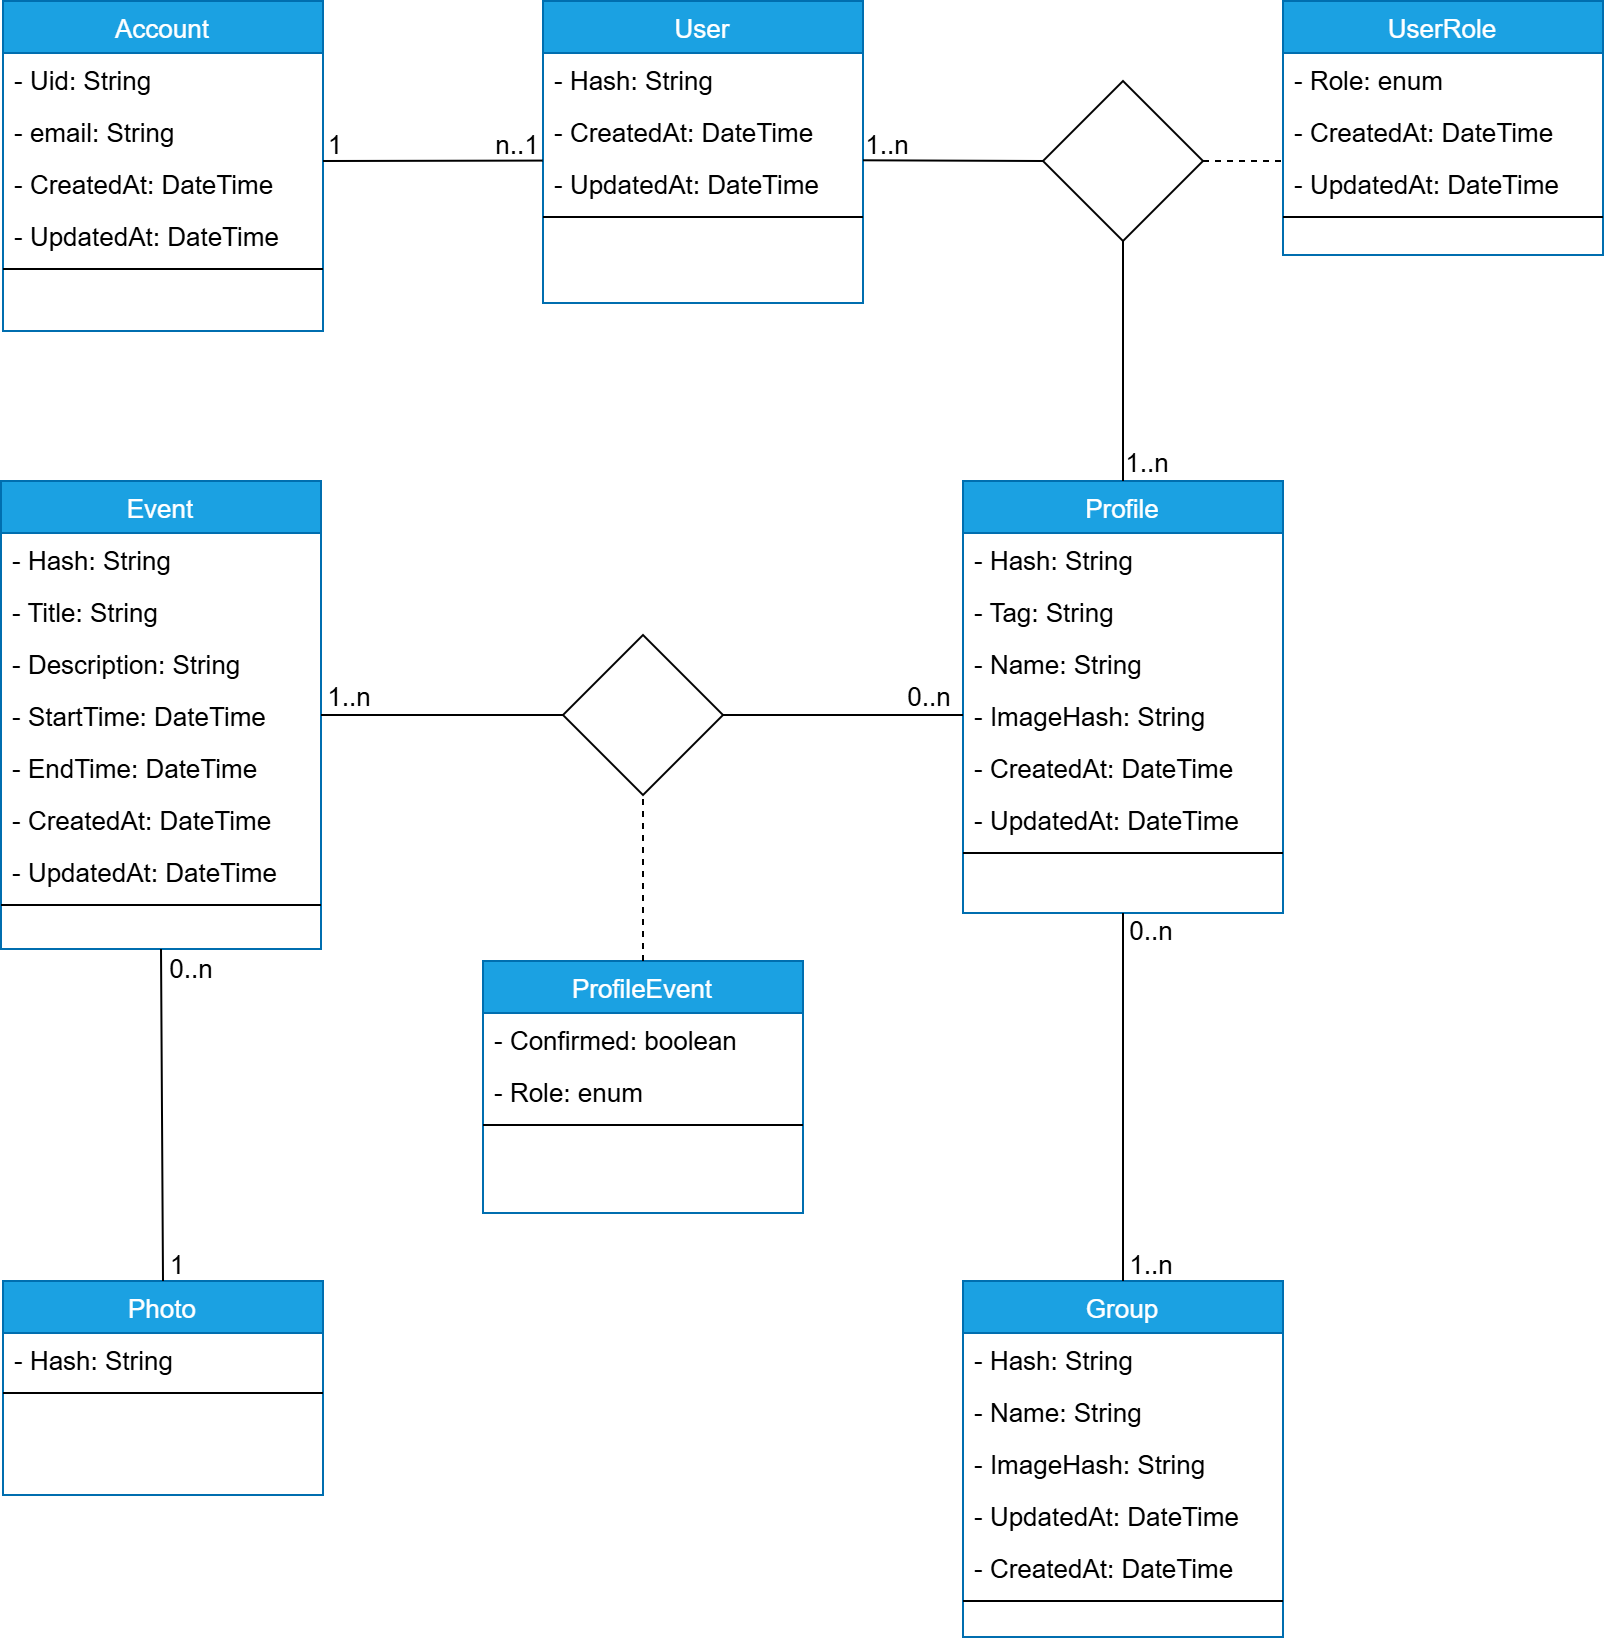
\includegraphics[width=\textwidth]{ProgettoDominioServer.png}
    \caption{ Diagramma del dominio}
\end{figure}
Le richieste riguardo alle informazioni tra Account, User e Profile, con i relativi UserRole, vengono eseguite all’avvio del programma, per poi essere mantenute in memoria locale. Le modifiche a questi elementi sono sporadiche.
Allo stesso modo gli oggetti Group vengono recuperati solo all’avvio dell’applicazione, e, salvo rari aggiornamenti, non occupano ulteriormente lo spazio delle richieste.

La maggioranza delle richieste verterà sull’ottenimento dei dati relativi agli Event e ai Profile. Infatti ad ogni avvio dell’applicazione sarà richiesto di recuperare gli eventi di ogni profilo, mentre, ogni volta che si apre il dettaglio di un evento, sarà necessario recuperare i rispettivi dati, includendo i profili associati. Si prevede che la cardinalità dei profili associati ad un evento risieda nell’ordine delle decine, mentre agli eventi che si associano ai profili l’ordine di grandezza previsto risiede nelle migliaia. 

La relazione che accomuna Event e Profile è di tipologia molti a molti, identificata con l’oggetto ProfileEvent. L’elemento ProfileEvent, oltre a descrivere la relazione, contiene la proprietà Confirmed, che indica la conferma di partecipazione di un profilo ad un evento. Vista la natura del progetto, la proprietà Confirmed, assieme ai dati degli Event, sarà tra i campi che subiranno modifiche con maggiore frequenza.

Riassumendo, le operazioni principali che vertono sulle prestazioni del database sono il recupero degli eventi relativi ai profili, il recupero dei profili collegati agli eventi, l’aggiornamento dei campi degli oggetti Event e la modifica del campo Confirmed relativa ai ProfileEvent.

Nonostante sia più probabile che venga richiesto il dettaglio di un evento, e quindi sia più frequente il dover recuperare i Profile relativi all’Event, la proporzione delle richieste prevista non giustifica lo sbilanciamento della relazione sugli Event.
Infatti, se si salvassero tutti i ProfileEvent sull’oggetto Event, le richieste degli eventi appartenenti ai profili, sebbene meno frequenti, richiederebbero l’ispezione di tutti gli Event alla ricerca del Profile indicato. 
Infine, se si duplicasse l’oggetto ProfileEvent, oltre che nella sua tabella originaria, anche sugli Event la sua creazione, la sua eliminazione e la modifica del campo Confirmed richiederebbero il doppio delle scritture.

Vista quindi la necessità di letture frequenti da entrambe le parti di una relazione molti a molti e la necessità di scrittura dell’oggetto che la identifica, si individua in un database relazionale la soluzione più efficace per il dominio del progetto. Infatti, i database relazionali sono ottimizzati sulle operazioni di unione tra tabelle, garantendo velocità di recupero in lettura da entrambe le parti. Permettendo la separazione delle tabelle e gestendo gli oggetti ProfileEvent come entità indipendenti, la modifica del campo Confirmed comporta il blocco del solo elemento ProfileEvent. Le caratteristiche ACID forniscono inoltre uno stato centrale per tutta l’applicazione, che, per quanto non strettamente necessario, garantisce l’uniformità delle informazioni per tutti gli utenti.
\clearpage
\subsubsection{Scelta del database}

Azure offre un’ampia scelta di database relazionali che possono essere integrati con il resto dell’ecosistema. Oltre alla tecnologia proposta, nella scelta del database più adatto bisogna considerare soprattutto l’integrazione con servizi accessori, le particolarità del server su cui viene eseguito, e i costi che si andrà ad affrontare.

\begin{figure}[h!]
    \centering
    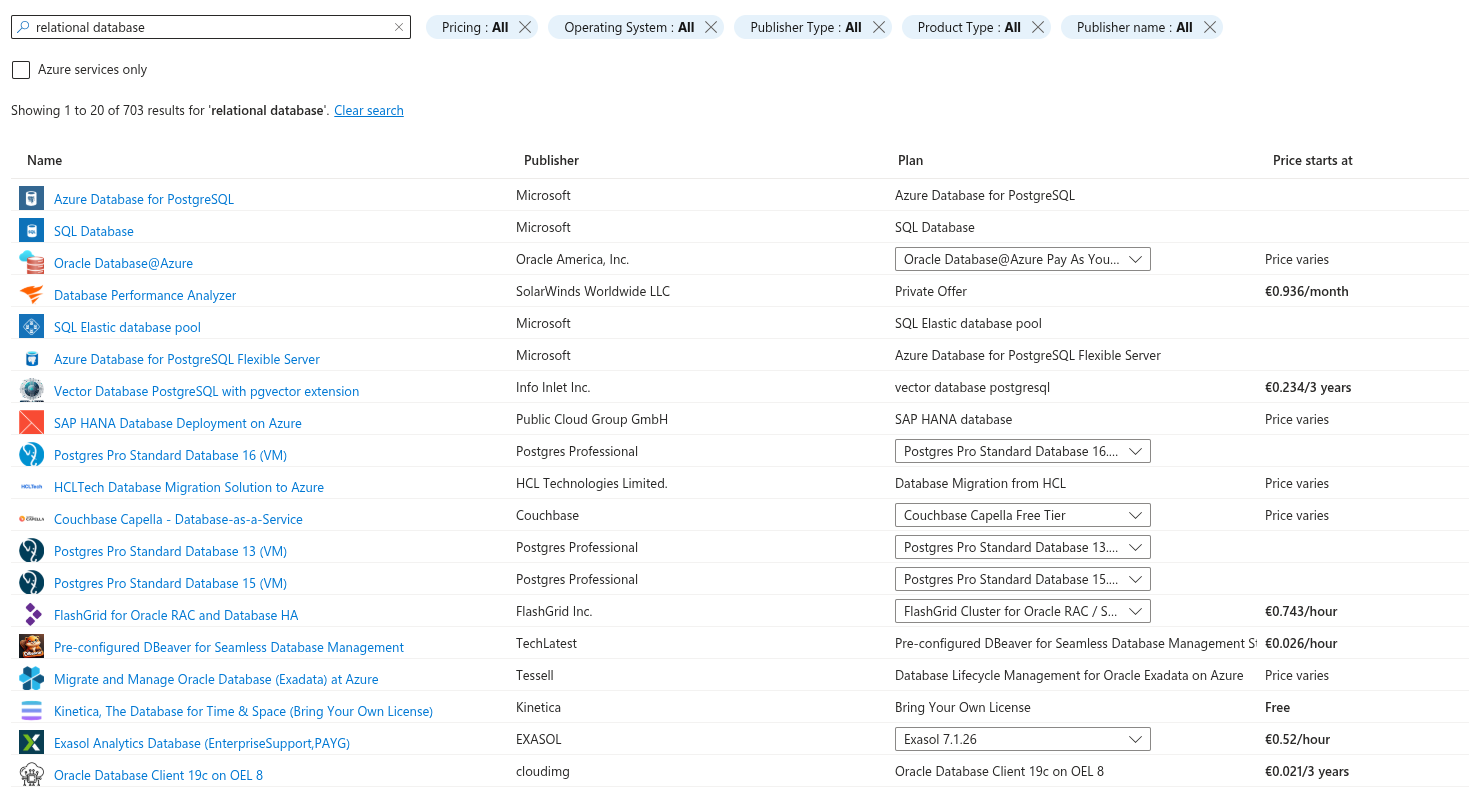
\includegraphics[width=\textwidth]{Possibilitadelcloud.png}
    \caption{Proposte di Azure per i database relazionali}
\end{figure}	


A meno di necessità particolari che richiedono l’utilizzo di una tecnologia implementata da uno specifico database, la grande sovrapposizione di funzionalità delle diverse offerte di database relazionali presenti sul mercato garantisce il  soddisfacimento delle necessità rilevate dall’analisi del dominio indipendentemente dalla tecnologia proposta dal servizio.

La grande differenza tra i vari servizi sta nelle proprietà del server incaricato di fornire il potere computazionale necessario per l’esecuzione. L’architettura del server e la sua integrazione con la tecnologia del database, infatti, determinano l’effettiva capacità di scalabilità del servizio. 

Si intende scalabilità verticale la capacità di aumentare le risorse della stessa macchina in cui si esegue il codice. La scalabilità verticale viene definita nel momento di creazione del servizio, in cui si determinano le risorse da dedicare alla macchina che esegue il programma. Trattandosi di macchine virtualizzate, è sempre possibile in un secondo momento aumentare le prestazioni in caso di necessità.

Per scalabilità orizzontale si intende invece la capacità di delegare il carico di lavoro ad altre macchine, eventualmente coordinando le modifiche. Questo permette una risposta alle richieste più resistente, riducendo il rischio di colli di bottiglia che potrebbero venirsi a formare nell’utilizzo di un nodo singolo.
La scalabilità orizzontale richiede però l’implementazione di tecnologie apposite integrate con il database che permettano l’esecuzione in nodi fisici differenti. 

Una volta individuata la tecnologia adatta e il livello di scalabilità desiderati, è bene considerare le altre necessità o le opportunità aggiuntive generate dalla presenza di un database nel progetto. 

L’alta disponibilità(HA) è la proprietà di garantire l’accesso al servizio nonostante i guasti. Ad esempio, si può mantenere una macchina identica al server principale in grado di replicare il servizio, spostando il carico in caso di guasto del server principale. Si misura in “numero di nove”, ovvero la quantità di nove presenti nella percentuale del tempo per il quale si garantisce la disponibilità del servizio.
I servizi offrono diverse qualità di HA, in base alle funzionalità desiderate.

Alcuni servizi possono presentare offerte di backup per riportare il server nello stesso stato di qualche momento precedente. Questo permette il ripristino del sistema ad un punto precedente rispetto all’avvenimento di eventuali errori o guasti del sistema.

Inoltre, Azure mette a disposizione molteplici servizi accessori che possono essere uniti al servizio. Questo permette di estendere le potenzialità del database tramite  l’analisi e il monitoraggio dei dati, generando prestazioni aggiuntive o integrando i dati per lo sviluppo di altre tecnologie.

Infine è necessario controllare i costi che le scelte progettuali e prestazionali hanno comportato: pur generalmente legati al consumo effettivo delle risorse, e quindi in grado di fornire solo una previsione del costo finale, ogni decisione presa conduce ad un possibile aumento di prezzo, ed è quindi bene controllare che le risorse selezionate siano effettivamente  necessarie a soddisfare i requisiti del progetto.

Riducendo al minimo i costi, visto l’utilizzo iniziale dell’applicazione, e nessuna necessità tecnologica specifica, la scelta del database per la persistenza del progetto è ricaduta su Azure SQL Database. 
Presentando un database relazionale di tecnologia proprietaria di Microsoft, Azure SQL database esegue su un solo nodo, fornendo però la possibilità di  scalare  verticalmente tramite la possibilità di modificare le risorse assegnate in ogni momento, garantendo comunque prestazioni soddisfacenti per il servizio.
Al server principale è stata affiancata una replica che rimane costantemente aggiornata. Situata in una località differente dal server principale, garantisce alta disponibilità continuando a fornire i servizi anche in caso di malfunzionamenti al server principale.
\subsubsection{ Limitazioni dei database relazionali}

La scelta di un database relazionale può però comportare limitazioni a livello prestazionale. Il più grande tallone d'Achille dei database relazionali è il numero limitato di connessioni contemporanee permesso. Questo comporta un numero massimo di richieste in contemporanea che il database può gestire, minacciando la scalabilità. 

Per ovviare ai problemi di scalabilità ci sono diverse soluzioni non esclusive che possono migliorare le prestazioni. Sicuramente si deve limitare al minimo il tempo in cui ogni richiesta mantiene la connessione, distinguendo nel codice momenti precisi e definiti in cui vengono richieste le modifiche al database.   

Inoltre, si può interporre un livello di caching tra la logica applicativa e le richieste al database. Il livello di caching si occupa di gestire le richieste al database fornendo e duplicando le risposte che possiede già in memoria, eventualmente centralizzando le richieste in caso i dati siano invece da recuperare. Per i dati in scrittura, invece, salva temporaneamente le modifiche richieste, aggiornando subito la memoria locale, per poi apportare le modifiche al database in momenti di carico ridotto. Garantisce così un tempo di risposta e di propagazione degli aggiornamenti ridotto. Questo consente di alleviare le richieste al database, estendendo di molto le prestazioni fornite.

Nel caso in cui però fossero necessarie ulteriori prestazioni, se il dominio e i requisiti lo permettono, si può eventualmente delegare ad un database non relazionale le modifiche ai dati e alle relazioni che non necessitano delle qualità ACID ma richiedono un’alta frequenza di scrittura. 

Infine, se fosse necessario mantenere un database relazionale, per aumentare le prestazioni conviene cambiare architettura e adottarne una che supporti la scalabilità orizzontale, per suddividere il carico su più nodi.




\subsubsection{ Integrazione con C\#}

La scelta di un database relazionale per la persistenza ha comportato sviluppi progettuali precisi. In primis si rende necessario tradurre il dominio in componenti relazionali che possano essere espressi e salvati nelle tabelle del database.

\begin{figure}[h!]
    \centering
    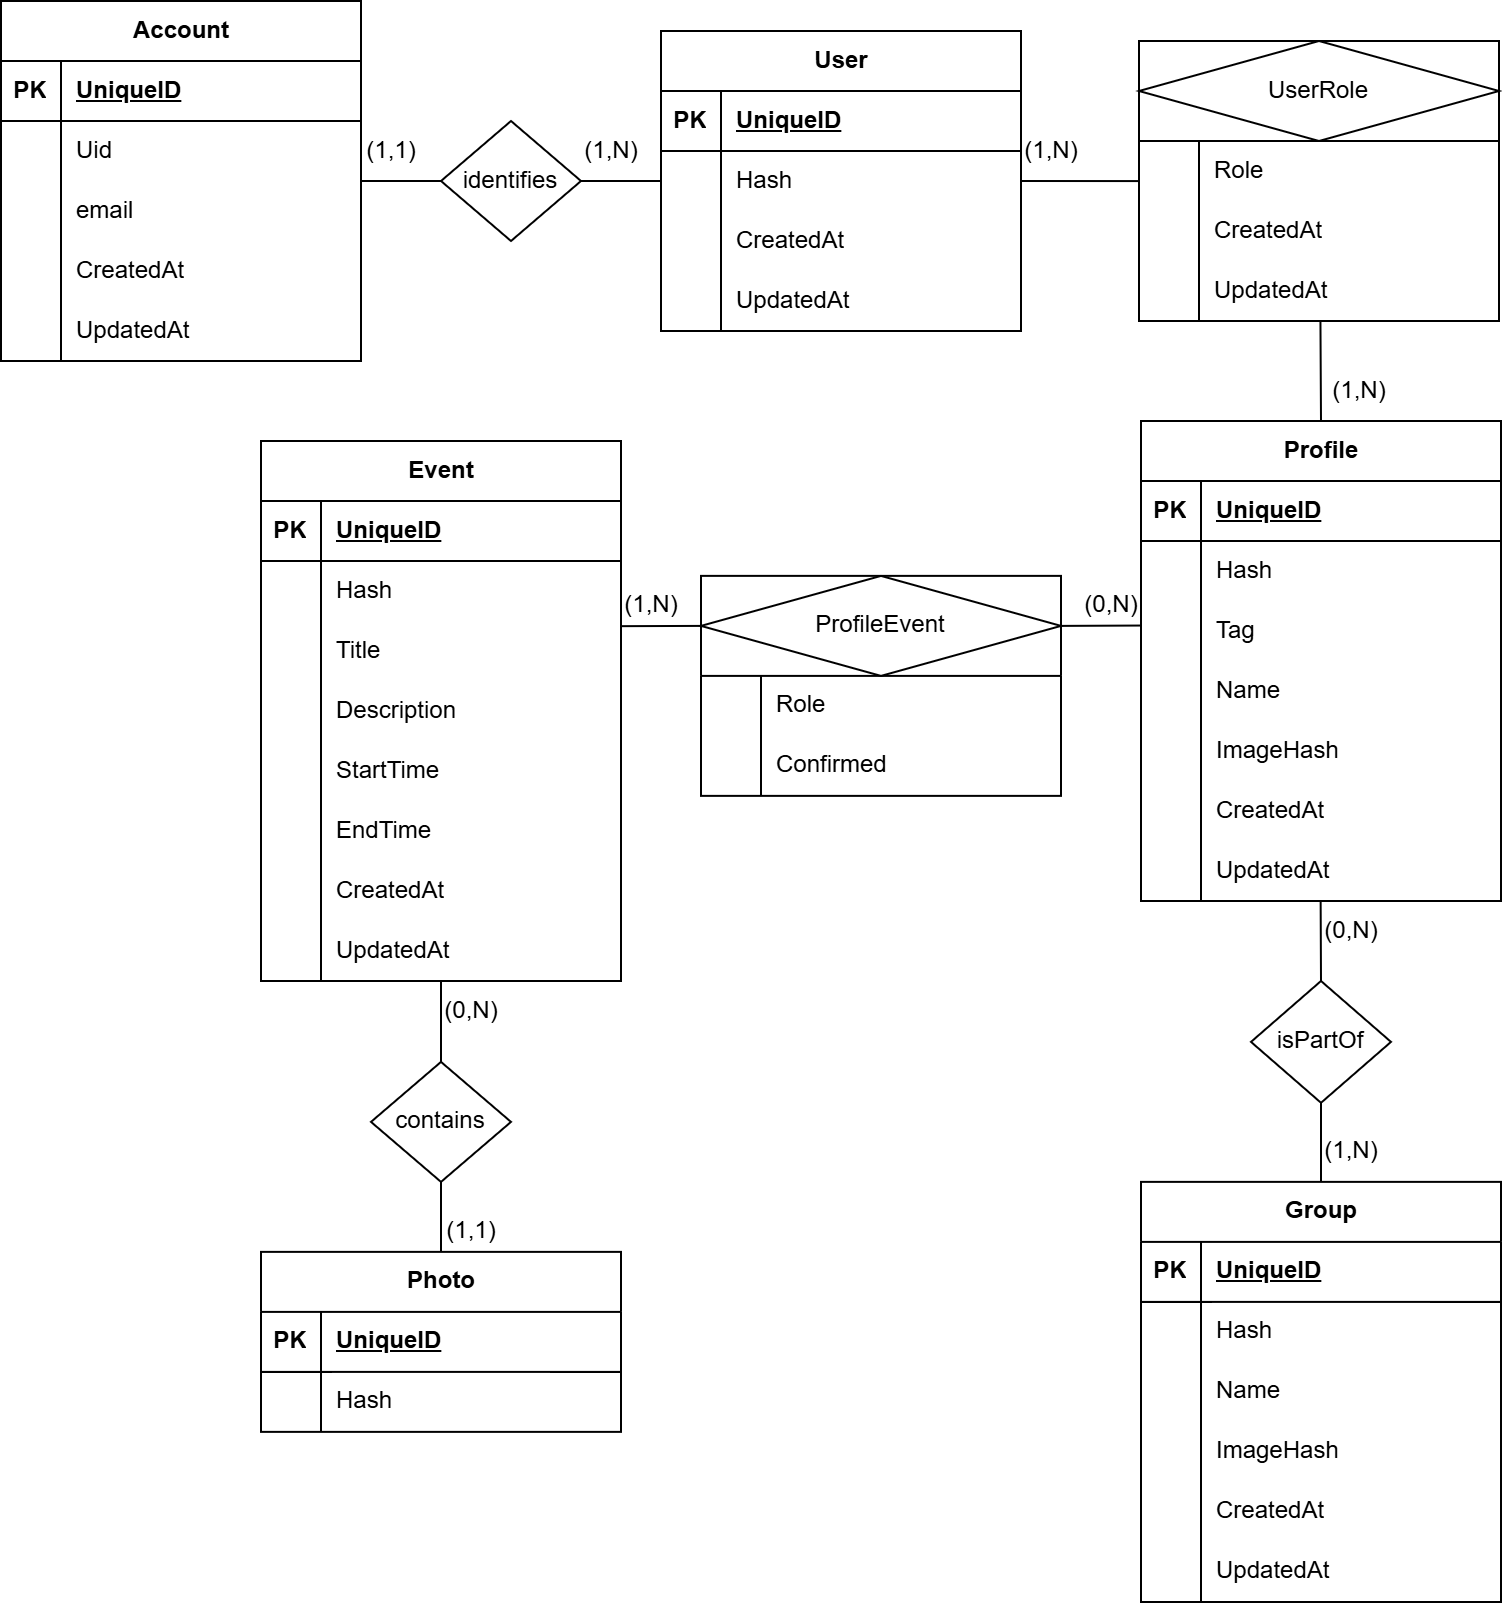
\includegraphics[width=\textwidth]{ProgettoDiagrammaER.png}
    \caption{Diagramma Entità - Relzione del dominio}
\end{figure}	

Si creano quindi sul server le classi logiche del programma, a partire dal dominio. Ogni classe corrisponde ad un oggetto del dominio, presentando i valori e le relazioni dei componenti come attributi dell’oggetto.




Entity Framework Core di .Net(EFCore) è una libreria di C\# che permette di unire le classi logiche del programma alle tabelle del database. Fornisce un’astrazione logica del collegamento con il database e le richieste relative, fornendo una rappresentazione di alto livello delle connessioni sottostanti. 


Una volta collegato il server con il database tramite le stringhe di connessione salvate sull’Azure Key Vault, sono state definite le proprietà tra le varie entità, per poi inizializzare in automatico la struttura del database. Le modifiche alla struttura del database vengono infatti generate automaticamente da EFCore in seguito alla creazione o alla modifica degli attributi degli oggetti. Questo permette di star dietro agli aggiornamenti, generando e salvando le modifiche da applicare ad ogni modifica delle proprietà del dominio.

Per la riduzione del carico computazionale richiesto da elementi con tante relazioni si utilizza la tecnica del lazy loading. La tecnica del Lazy Loading consiste nel richiedere i dati delle relazioni di un elemento solo quando strettamente necessario. La sua realizzazione tramite EFCore è attuata grazie alla proprietà virtual, che permette di gestire un oggetto con un riferimento al database richiedendo i dati delle sue relazioni solo quando viene espressamente richiesto.


\clearpage
\subsection{ Cache Locale}

Richiedere e ottenere dati dal server comporta ritardi che impattano sulle prestazioni. 
Se la tecnologia del dispositivo lo permette, è utile salvare copie delle informazioni usate più frequentemente nella memoria locale del dispositivo. Nel momento di una interazione che richiede la ricerca dei dati, si possono fornire le informazioni disponibili in copia, per poi eventualmente aggiornarle se si rivelassero imprecise. Questo permette un tempo di risposta apparente minore e una migliore esperienza utente.
\subsubsection{ Creazione della memoria locale}
Non tutti i dispositivi permettono una gestione della memoria a lungo termine. In particolare, i browser web non presentano questa funzionalità, ma i dispositivi mobili e i programmi si. 

Per motivi di prestazioni, il framework Flutter nativamente mantiene lo stato di un componente solo il tempo strettamente necessario per la sua esecuzione. Il tempo di vita dello stato coincide normalmente con quello del componente a cui è associato. La normale persistenza degli elementi e dei dati ha durata limitata. Si rende necessaria la creazione e la gestione di una cache locale che permetta di mantenere i dati ricevuti dal server anche in seguito al termine di servizio dei componenti.

\begin{figure}[h!]
    \centering
    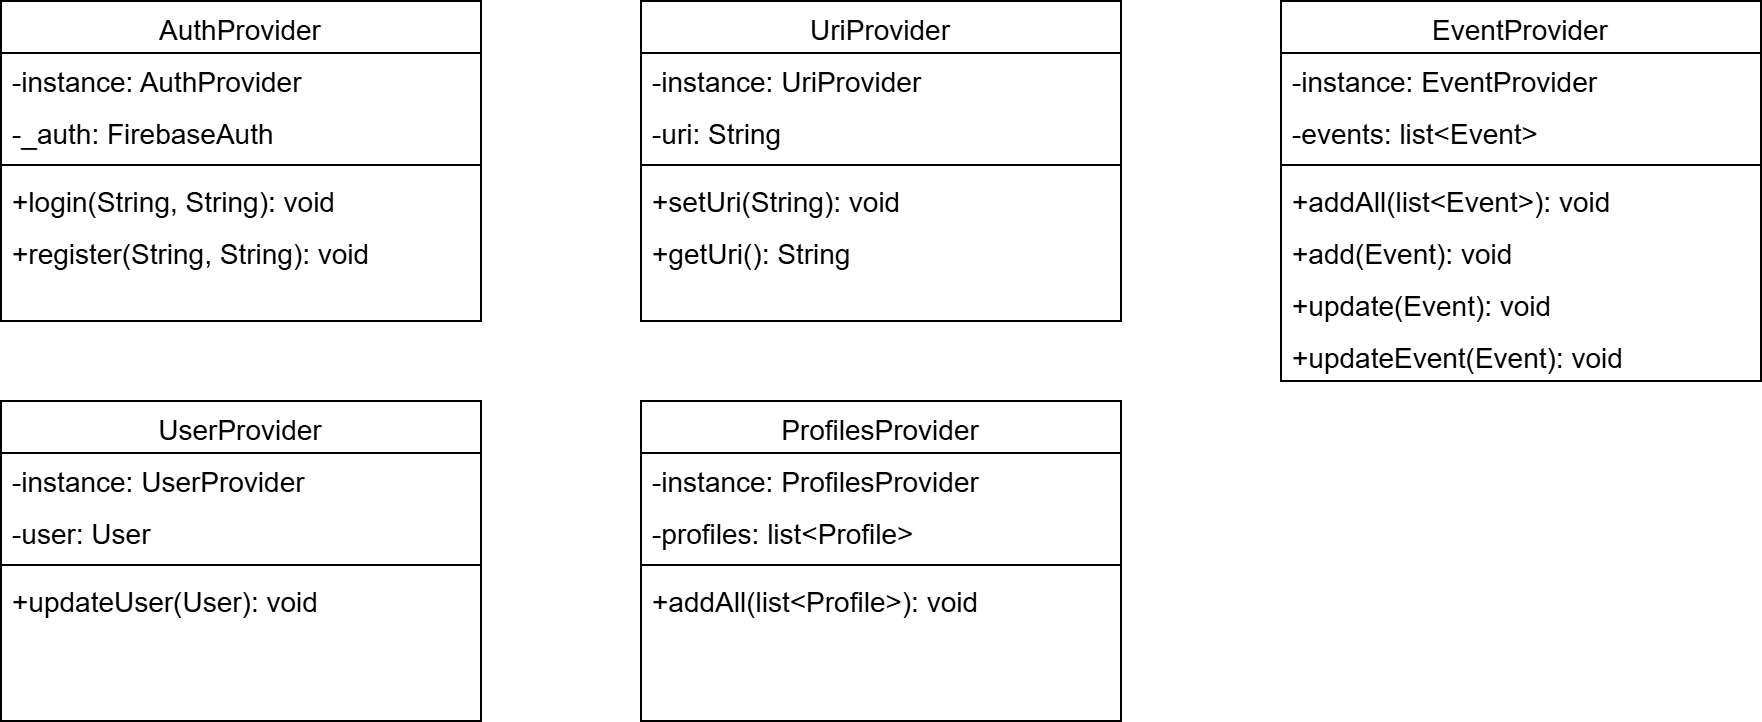
\includegraphics[width=\textwidth]{FrontProviderClassDiagram.png}
    \caption{Classi provider all'interno dell'applicazione}
\end{figure}	
La cache locale viene suddivisa in base alle classi logiche del dominio, ed è accessibile tramite servizi dedicati. In particolare, grazie a componenti di tipologia provider è possibile aggiornare in automatico le parti dell’applicazione interessate dalle modifiche. Al termine di una richiesta dati al server, il provider viene notificato, salvando il dato in memoria e scatenando un aggiornamento a catena sui componenti interessati.

La cache deve essere unica e disponibile in tutto il programma. 
I provider attraverso cui si realizza la cache locale seguiranno il pattern singleton, che garantisce l’unicità dell’elemento all’interno del programma. Una volta creati all’avvio del programma, infatti, tutti gli elementi dell’applicazione avranno accesso agli stessi dati, quando necessario.

\begin{figure}[h!]
    \centering
    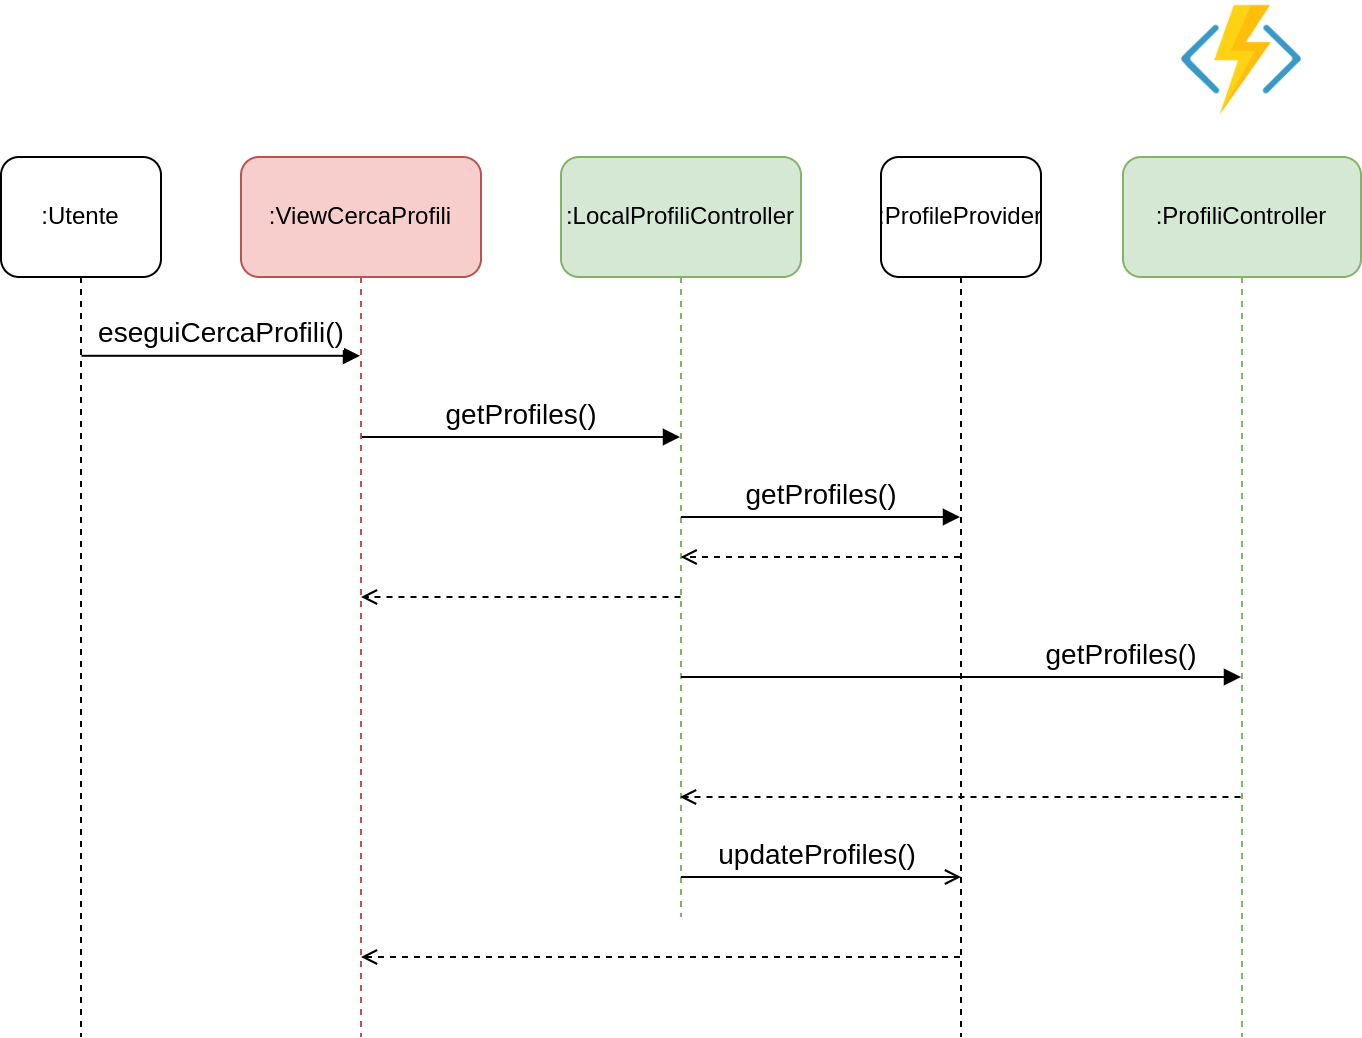
\includegraphics[width=\textwidth]{Providers.png}
    \caption{Esempio di interazione logica tra i componenti del client}
\end{figure}	

eventualmente salvataggio delle modifiche offline per caricarle quando si torna online. 

\subsubsection{ Allineamento con la memoria centrale}

il client ha la responsabilità di tenere allineata la propria cache ai valori della memoria centrale. Per quanto possa fare temporaneamente affidamento sulle risorse che ha salvato in cache per ridurre i tempi di risposta con l’utente, la loro validità dipende dalla certezza che corrispondano ai dati ufficiali. 

Ogni elemento avrà associato l’ultimo momento in cui è stato aggiornato. Allo stesso modo, viene salvato l’ultimo momento in cui è stata attivamente effettuata una richiesta esplicita di aggiornamento.  
Ad ogni avvio dell’applicazione il client invierà una richiesta al server per ricevere tutti gli elementi che hanno subito modifiche successivamente al momento dell’ultimo aggiornamento. 

La necessità di avere aggiornati tutti gli elementi della cache nel minor tempo possibile dipende anche dalla tipologia dell’elemento. Bisogna identificare gli elementi per il quale l’allineamento è critico per il corretto funzionamento dell’applicazione, come invece quelli che svolgono ruoli secondari e possono essere aggiornati anche in un secondo momento. Ad esempio, la modifica della durata di un evento è necessario venga rilevata il prima possibile, mentre la modifica della foto associata ad un profilo ha vincoli di aggiornamento in memoria locale molto più rilassati.

Nel caso di dati critici si implementa un meccanismo che esegue, periodicamente, una richiesta degli elementi modificati nell’arco di tempo dall’ultimo aggiornamento, per poi aggiornare il loro valore. Invece, nel caso di elementi secondari, si possono richiedere allineamenti direttamente nel momento in cui vengono posti espressamente in attenzione dato l’utilizzo dell’app.


\subsection{Aggiornamenti}

Data la natura condivisa dell’applicazione risulta fondamentale che gli utenti siano aggiornati in tempo reale sulle modifiche applicate agli eventi, oltre ad essere una prerogativa di tutte le applicazioni moderne, anche per migliorare la user experience. lo spostamento di un appuntamento, la conferma di una presenza o la modifica del luogo di appuntamento sono elementi critici che è bene che gli utenti vengano informati il prima possibile. 

Il cloud fornisce strumenti per il supporto e lo sviluppo di queste funzionalità, ma, oltre a dover individuare la tecnologia più adatta, bisogna anche essere in grado di integrarla nel resto del progetto.

\subsubsection{ Scelta della tecnologia}


La comunicazione con il server finora implementata si basa sul protocollo Hypertext Transfer Protocol (HTTP). HTTP prevede un fornitore di servizi (il server) mettere a disposizione una porta ad un indirizzo fisso rimanendo in attesa di eventuali utilizzatori (client) che, interfacciandosi attivamente alla porta disponibile,  espongono le loro richieste.
La riduzione delle comunicazioni al minimo indispensabile, oltre a non richiedere al server alcuna conoscenza del client, rende il protocollo pratico e scalabile.

Questa dinamica però impedisce ai client di essere notificati di eventuali modifiche apportate, a meno di richieste periodiche frequenti che comportano un sovraccarico da entrambe le parti. Inoltre, l’inversione dei ruoli non è applicabile in quanto i client cambiano costantemente l’indirizzo a loro associato, così come è impossibile distinguere se il dispositivo abbia terminato la connessione o se sia un guasto di altro tipo. 

Si necessita una comunicazione che mantenga in costante contatto i client con le modifiche del server, permettendo una trasmissione attiva degli aggiornamenti.
A basso livello, il protocollo che permette una comunicazione continua più adatto alle tecnologie comunemente diffuse è quello delle WebSocket. Tramite WebSocket infatti si crea un canale diretto tra le parti che consente una comunicazione istantanea. 

Alla necessità di supportare il protocollo delle WebSocket e di inviare istantaneamente i messaggi, si aggiunge la possibilità di creare molteplici canali specifici per indirizzare correttamente le comunicazioni ai soli interessati.


\begin{figure}[h!]
    \centering
    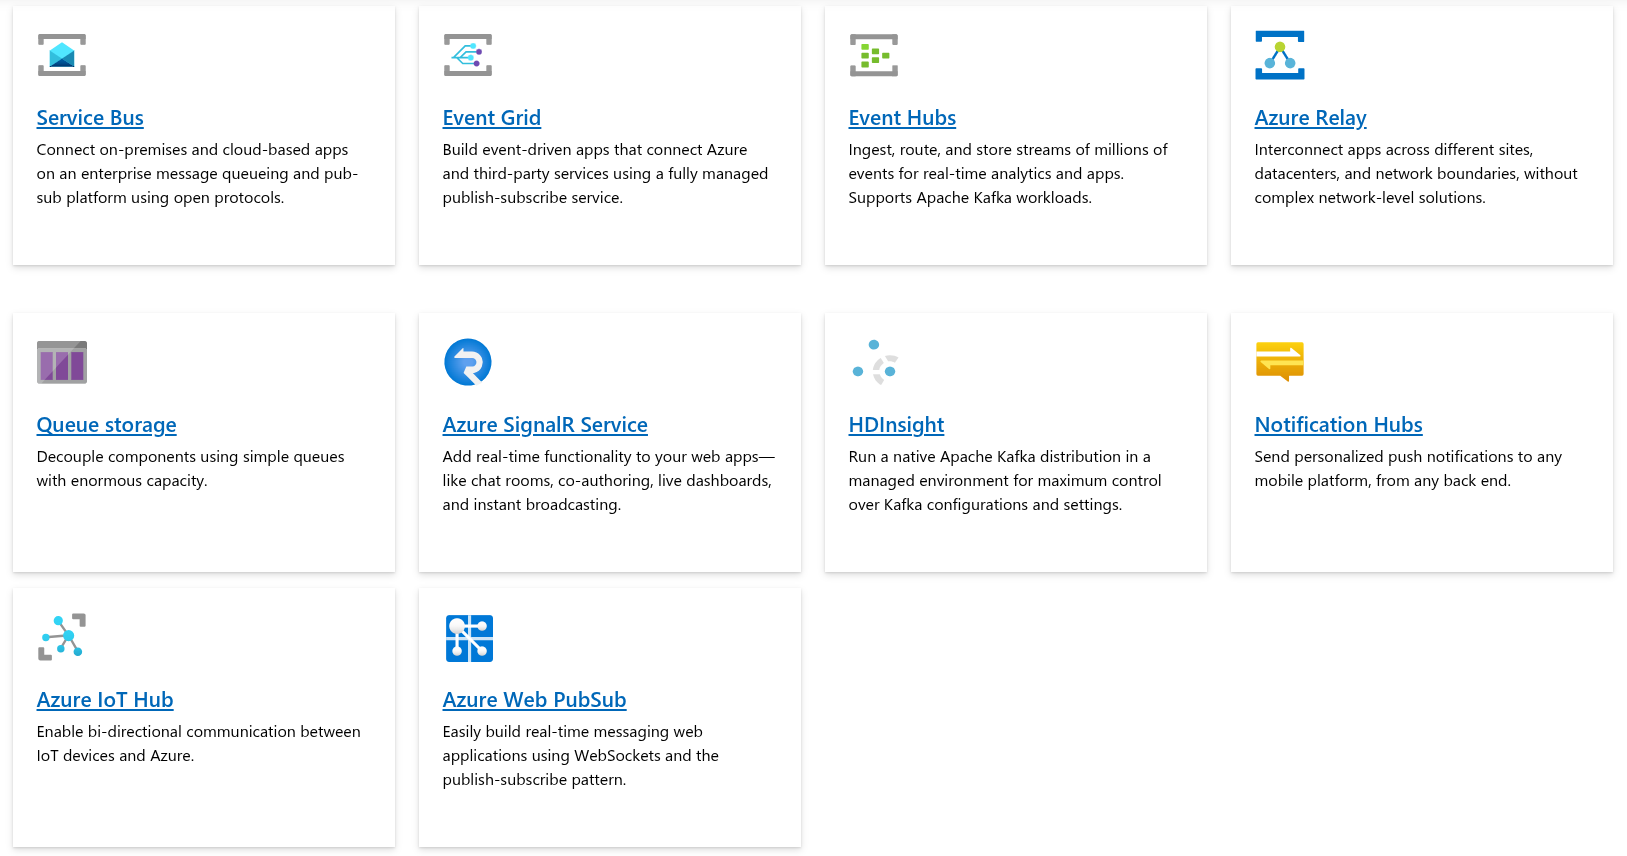
\includegraphics[width=\textwidth]{AzureMessagingServices.png}
    \caption{I servizi di comunicazione istantanea proprietari di Azure}
\end{figure}	


Per individuare la tecnologia più adatta ad aggiornare gli utenti, tra le tante che offrono servizi di collegamento istantaneo tra tecnologie, è fondamentale comprendere  gli scopi per cui sono nate e che problemi quindi risolvono. Infatti, ogni servizio è stato progettato per affrontare specifiche sfide che si differenziano sia per la natura dei servizi a cui si rivolgono che per  modalità di approccio .

La natura degli attori per cui il servizio si specializza determina le prestazioni di scalabilità e le integrazioni supportate. Bisogna quindi considerare la località e la natura delle risorse: in-premise o sul cloud, se appartengono alla stessa piattaforma o se devono comunicare internamente.
Ad esempio, un servizio pensato per collegare tantissimi dispositivi distribuiti con limitato potere computazionale, come nel caso dell’Internet of Things, fornirà  supporto a connessioni esterne e a protocolli standard, e prevederà un’elevata quantità di richieste di limitate dimensioni e frequenza. Viceversa, la necessità di creare una comunicazione tra un numero ristretto di server con prestazioni elevate comporta la creazione di flussi di dati importanti, magari gestiti internamente all’ambiente cloud, astraendo la tecnologia necessaria.

I servizi si differenziano però anche per le caratteristiche delle connessioni gestite.
Proprietà fondamentale è la natura delle comunicazioni. I canali possono essere infatti unidirezionali, permettere la comunicazione da entrambe le parti o implementati come flussi di eventi, in cui le comunicazioni possono essere inviate e ricevute da molteplici attori, senza che il destinatario sia noto al mittente. Inoltre, alcuni servizi offrono la possibilità di individuare categorie di clienti specifiche a cui eventualmente inviare notifiche mirate. Infine, bisogna prendere in considerazione la necessità di persistenza delle comunicazioni, che fornisce, oltre all’aggiornamento in tempo reale, anche la possibilità di recuperare modifiche passate.

Nel progetto si necessita di un servizio che supporti le WebSocket e che permetta di creare una molteplicità di canali unidirezionali differenti. In particolare, deve essere il più indipendente possibile dagli attori con cui comunica per poter garantire il maggior supporto possibile. Dovendo coprire solo le notifiche di aggiornamento, senza responsabilità di rintracciabilità dei dati, la presenza della persistenza non è necessaria.

Gratuito per le prime 20 connessioni, ma eventualmente scalabile per soddisfare ulteriori carichi, il servizio individuato per la gestione delle notifiche in tempo reale è Azure Web Pub Sub (AWPS). Permette infatti la creazione di canali tramite WebSockets e l’integrazione con le Azure Function. Supporta la creazione di canali, sia unidirezionali che bidirezionali, su cui pubblicare eventi, a cui gli utenti possono collegarsi per ricevere gli aggiornamenti. Non prevede l’utilizzo di persistenza ma gestisce completamente la scalabilità e l’affidabilità del sistema.



\subsubsection{Integrazione}

L’integrazione di Azure Web Pub Sub deve avvenire sia con il server che con i devices degli utenti. Seguendo il modello publish subscribe, ogni client si connetterà ad un canale in sola lettura, ricevendo tutti i dati che verranno pubblicati su di esso. Il server avrà il compito di interfacciarsi con il servizio per pubblicare i dati sui canali interessati.

La scelta della definizione del canale deriva da un’ulteriore analisi del dominio. 
Il soggetto interessato alle modifiche sottoposte a notifica è il profilo. 
Se però si creassero i canali in relazione ai profili ogni dispositivo (che riassume l’interazione di un utente) dovrebbe mantenere una connessione per ogni profilo collegato all’utente. La creazione di un canale per ogni device allo stesso modo risulta estremamente inefficiente, in quanto, oltre ad introdurre nuovi requisiti per garantire la tracciabilità dei dispositivi, ne richiederebbe di creazione e gestione in numero elevato. Per queste ragioni i canali verranno creati uno per utente, garantendo inoltre che gli unici utenti a ricevere le notifiche ne posseggano effettivamente l’accesso adeguato.

A seguito di una richiesta che comporta la notifica ai profili interessati, il server avrà il compito di interfacciarsi con AWPS per affidargli le comunicazioni relative. Tuttavia AWPS non supporta la capacità di unire gli elementi in base alle loro relazioni, per cui la responsabilità di trovare gli utenti interessati ricade sul server. 
Ad esempio, la modifica di un evento comporta la notifica a tutti i profili relativi, e quindi una comunicazione a tutti gli utenti che ne posseggono i permessi di notifica per la particolare azione su detti profili. 

L’operazione di ottenimento degli utenti coinvolti data l’azione svolta (nell’esempio, la modifica di un evento) verrà eseguita in un’altra Azure Function dedicata che si occuperà poi, per ogni utente coinvolto, di comunicare  al server AWPS il messaggio da notificare. L’eventuale fallimento della operazione viene inserito tra i log e risulterà durante i monitoraggi, senza coinvolgere la funzione principale.

		
\begin{figure}[h!]
    \centering
    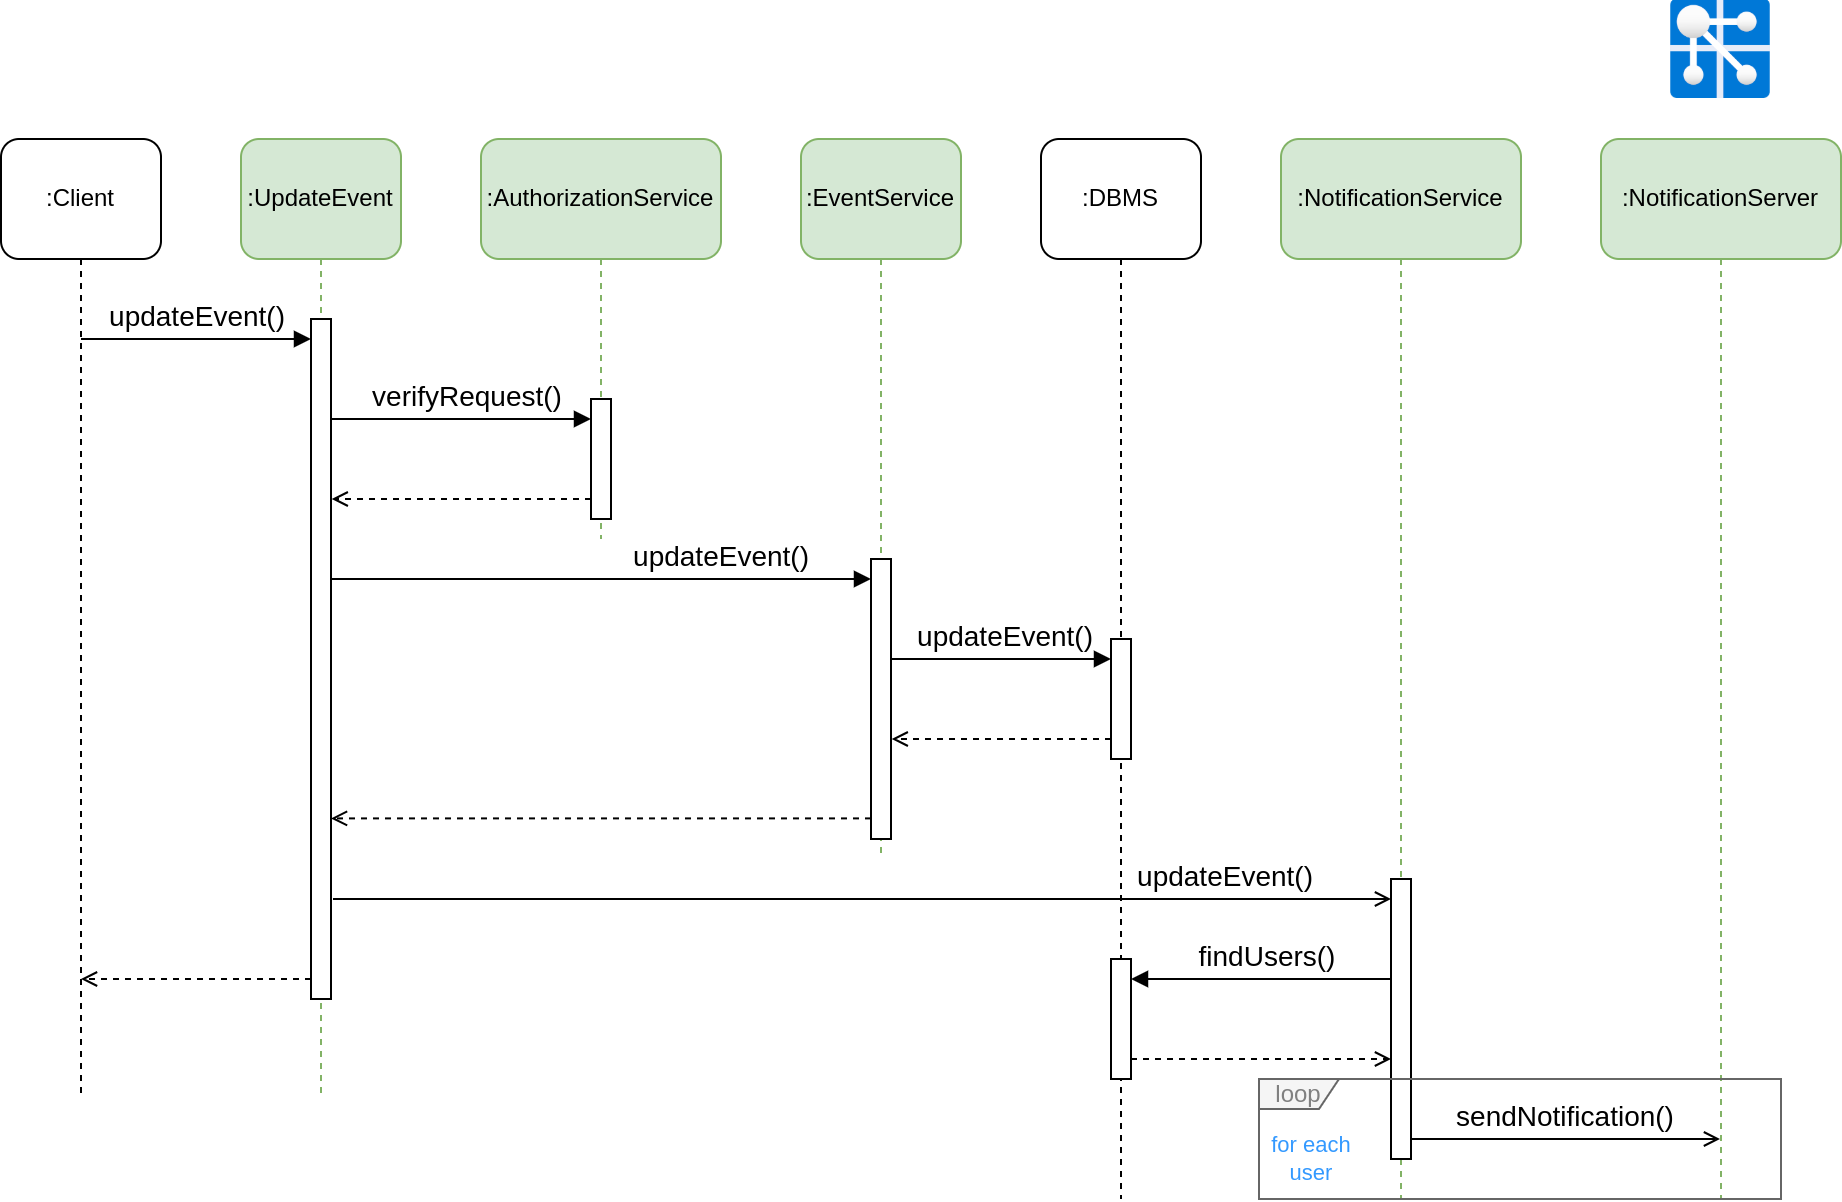
\includegraphics[width=\textwidth]{IIModificaEvento2.png}
    \caption{Interazione delle Azure Functions con AWPS}
\end{figure}	

La ricezione della notifica sul dispositivo dell’utente può comportare la richiesta al server dell’elemento modificato. La scelta di recuperare i dati tramite il server invece di includere i dati direttamente all’interno della notifica permette di uniformare il formato delle notifiche, semplificando la loro gestione e velocizzando l'invio; di diminuisce il volume dei dati trasmessi tramite WebSocket, garantendo la scalabilità delle notifiche; di migliorare la gestione degli errori da parte del server rendendoli più affidabili e di garantisce la possibilità di recuperare solo l’ultimo aggiornamento, riducendo il consumo totale dei dati.


\begin{figure}[h!]
    \centering
    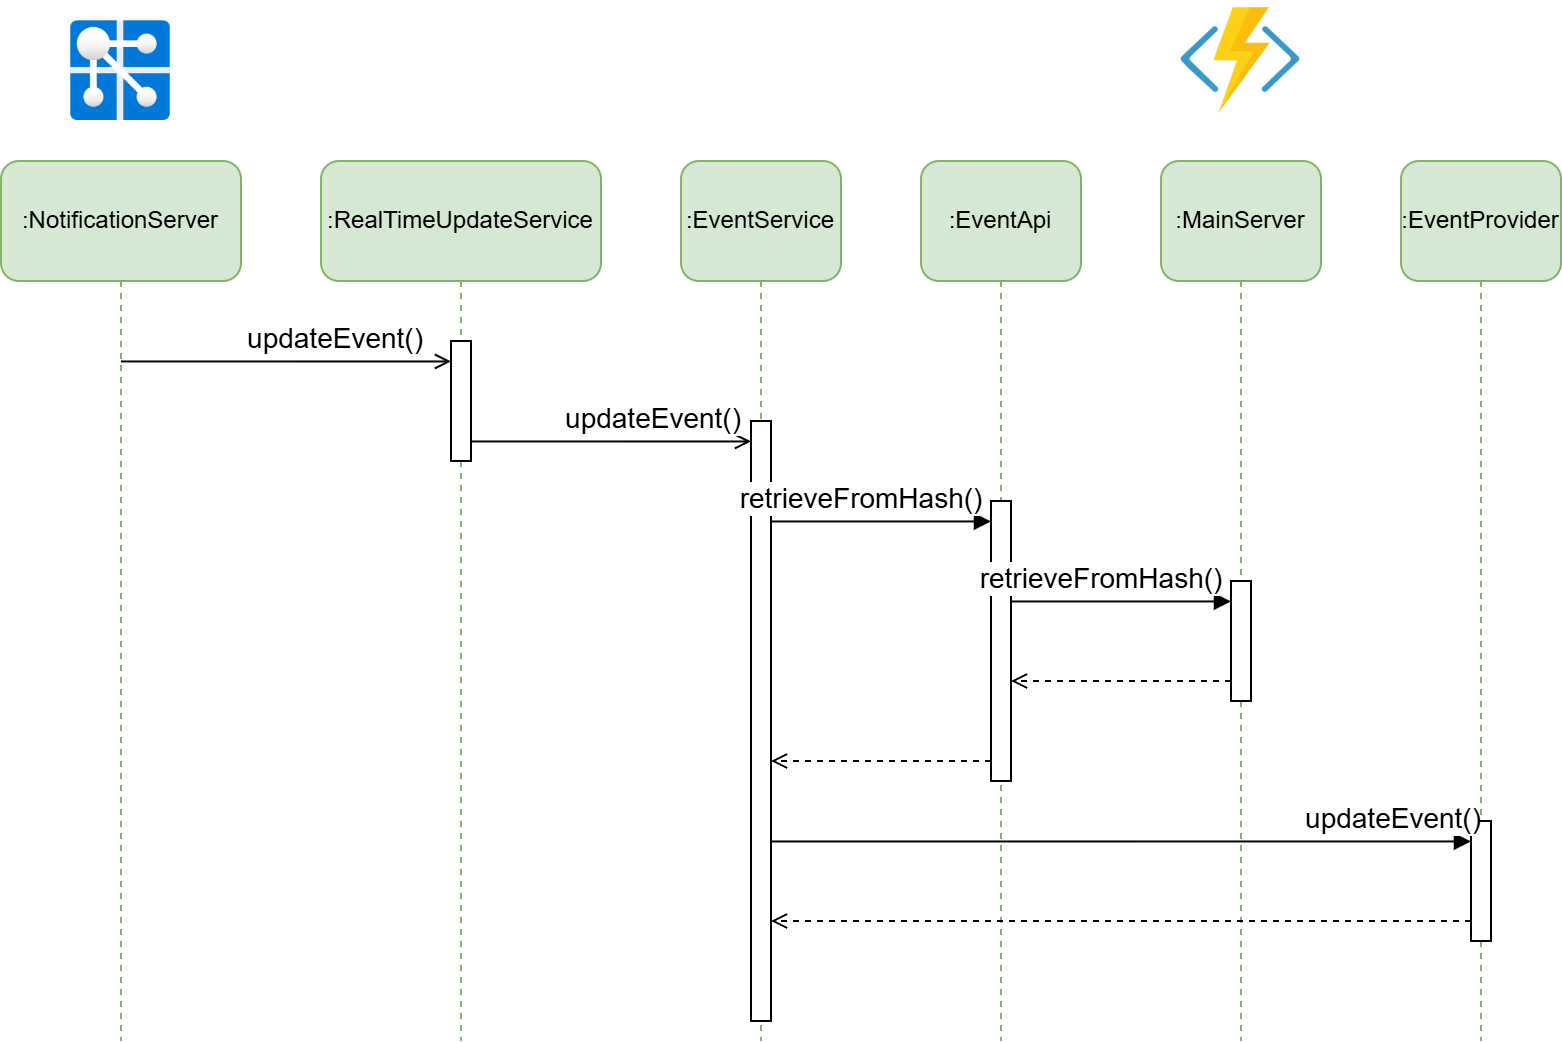
\includegraphics[width=\textwidth]{IIAggiornaEvento.png}
    \caption{Interazione tra AWPS e un client}
\end{figure}	

\clearpage
\section{Gestione dei dati Multimediali}
	
\clearpage

	
\subsection{ Recupero} 

L’aggiunta delle immagini richiede prima una fase di recupero. L’utente ha la possibilità di selezionare direttamente le immagini dal dispositivo utilizzato. In alternativa, sui dispositivi mobili, il sistema implementa una logica per rilevare automaticamente le foto scattate durante l’evento.

La possibilità di analizzare la galleria del dispositivo alla ricerca delle foto sussiste solo a seguito del permesso esplicito da parte dell’utente. Al primo accesso dell’applicazione verrà quindi richiesto il permesso all'accesso alla galleria, seguito dalla richiesta di poter creare notifiche. In caso tale concessione fosse negata, verrà richiesto ogni qual volta fosse reso necessario.

A seguito del termine di ogni evento, nel primo momento utile, l’applicativo esegue una ricerca delle foto scattate durante la sua intera durata. Nel caso in cui siano state rilevate immagini, vengono salvati i loro riferimenti in memoria locale, per poi notificare l’utente del loro ritrovamento. L’utente può quindi modificare la selezione, confermando o meno il caricamento delle foto trovate.



\begin{figure}[h!]
    \centering
    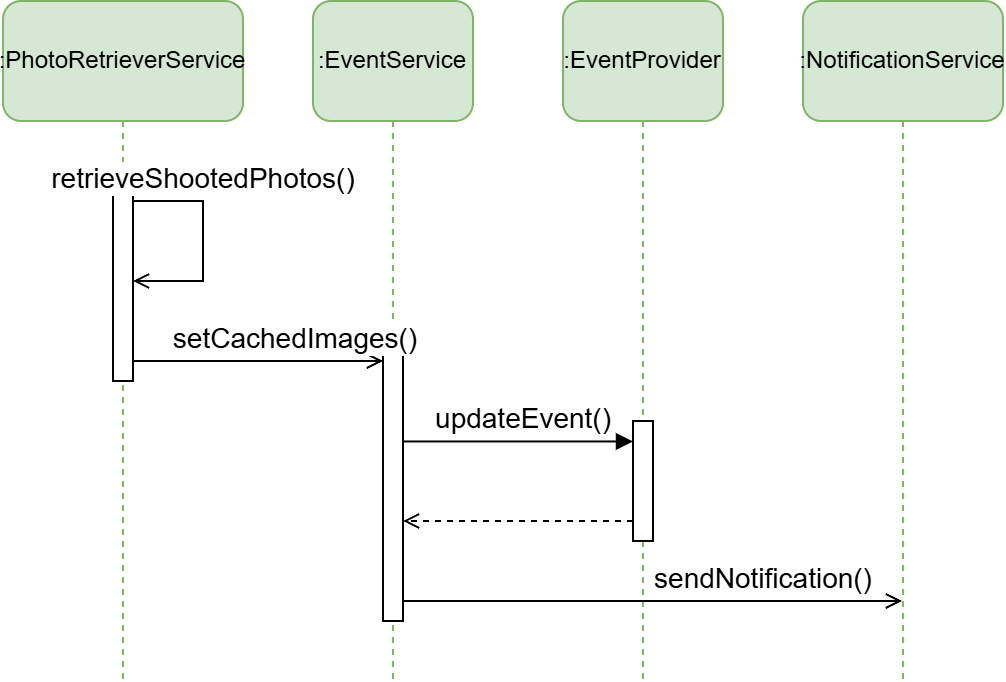
\includegraphics[width=\textwidth]{IIRecuperaImmagini.png}
    \caption{Interazione tra i componenti per il recupero delle immagini}
\end{figure}	





Pur risultando fondamentale per fornire un servizio trasparente con gli utenti, limitando disguidi e rischi dovuti ad un utilizzo inappropriato, la fase di conferma dell’utente presenta anche vantaggi prestazionali, mentre non costituisce un obbligo di natura legale. 

Le procedure di selezione e di recupero automatico delle immagini dalla galleria dell’utente sono contenute nelle modalità d’uso che l’utente deve accettare espressamente. Come previsto dalla normativa di tutela dell’immagine (C.C. art.10 e L. n.633/1941 artt. 96-97) e della privacy (GDPR: Reg.to UE 2016/679), la responsabilità per la pubblicazione delle immagini è in capo a chi realizza la foto, che ha l’obbligo di chiedere il consenso al/ai soggetti presenti nell’immagine. 


Come già affrontato nel capitolo precedente, richieste che prevedono la modifica di uno stesso componente comportano vincoli di concorrenza per l’accesso alla risorsa interessata. Il termine di un evento condiviso con più utenti crea il rischio  della ricezione contemporanea di più richieste di aggiunta di immagini convergenti sullo stesso elemento. L’attesa della selezione introduce un ritardo tra la fine dell’evento e il caricamento delle immagini interessate. La differita comporta una diffusione delle richieste maggiore nel tempo, riducendo l’eventualità di collisione di due richieste sullo stesso evento.

Al termine della selezione, le immagini verranno inviate al server, per essere salvate e allegate all’evento. 


\subsection{ Salvataggio}

A differenza dei dati normalmente scambiati, i file multimediali presentano dimensioni significativamente superiori, con differenze che si manifestano su ordini di grandezza rilevanti. 

Un salvataggio allineato ai dati degli elementi logici comporterebbe un rallentamento di tutte le operazioni, con impatto significativo sulle prestazioni del sistema. Si necessita quindi una gestione della memoria creata appositamente. 
Le dimensioni delle immagini e dei video influenzano inoltre il tempo di elaborazione e il volume delle richieste, richiedendo risorse maggiori a tutti i componenti del sistema. Infine, vista la possibilità di allegare più file ad un evento, il tempo maggiore di caricamento delle immagini potrebbe portare a tempi lunghi di transazioni per le modifiche degli eventi.


\subsubsection{Persistenza}

La visualizzazione dei file multimediali ricopre una priorità minore rispetto alle altre funzionalità offerte dall’applicazione. Si può quindi accettare un maggior tempo di caricamento se questo comporta una riduzione della latenza delle altre operazioni. Il salvataggio dei file multimediali sul database centrale aumenterebbe significativamente il volume specifico delle richieste, comportando un maggiore impiego di risorse computazionali e un aumento dei tempi di caricamento. Tale fenomeno potrebbe incidere negativamente sulle prestazioni complessive del sistema, penalizzando l'esecuzione simultanea di altre operazioni.

Attraverso la separazione dell'oggetto logico dal suo valore binario, si può distinguere la relazione tra il file e l'evento dai dati binari che lo compongono. Una volta recuperati i riferimenti ai file multimediali associati all’evento, sarà quindi possibile ottenere i loro valori binari in un secondo momento. Il modello del dominio visto in precedenza mostra la relazione logica tra l’evento e i file associati(Photo).
Data necessità e la possibilità di salvare i dati dei file multimediali su risorse differenti rispetto al database centrale, occorre individuare la soluzione più adatta per la loro persistenza.

Le principali tipologie di servizi in cloud per il salvataggio dei file multimediali si suddividono in Object, File e Block Storage.

Gli Object Storage gestiscono i file su un unico livello, con la possibilità di aggiungere metadati agli oggetti.  Ad ogni elemento viene associato un codice univoco attraverso il quale sarà possibile recuperarlo. L’accesso ai dati avviene generalmente tramite API RESTful, che oltre a dare la possibilità di gestire permessi, permette l’utilizzo su ampia scala. L’unico livello di indirizzamento permette una scalabilità illimitata, e il prezzo varia solo in base alla quantità dei dati salvati. 

I File Storage organizzano i file in una struttura gerarchica di cartelle e sottocartelle, che consente una maggiore facilità di accesso e gestione dei file. La particolarità della struttura permette un controllo ulteriore dei permessi degli utenti, inoltre fornisce la compatibilità con protocolli di accesso basati sui file systems, permettendone l’integrazione con tecnologie particolari. La scalabilità di questa tecnologia dipende molto dall’organizzazione dei file, e dalla loro quantità. La sua capacità dipende dal piano selezionato, così come il prezzo.


I Block Storage gestiscono la memoria tramite blocchi logici di dati, salvati separatamente con identificatori univoci. I blocchi vengono associati a volumi che ne permettono l’interazione, fornendo la possibilità di variare la tipologia di interazione con i blocchi. Permettono ampie prestazioni di recupero e modifica dei dati ma le prestazioni variano in base alla quantità di dati presenti. La scalabilità è limitata alla capacità assegnata al volume. Il prezzo è elevato, soprattutto per grandi moli. 

La tecnologia più adatta al salvataggio dei file multimediali del progetto è di tipo Object Storage. Assicurando una scalabilità infinita, risponde alla necessità di salvare grandi quantità di elementi con una scarsa relazione tra loro. L’identificazione univoca permette un'alta velocità di ritrovamento dei dati, così come la risposta prestazionale a numerose richieste contemporanee.

Il servizio di Object Storage fornito da Azure è Azure Blob Storage (ABS). ABS prevede un'organizzazione centrata su entità logiche Container che raggruppano più file multimediali, introducendo un livello di indirizzamento aggiuntivo. Permette l’accesso in lettura tramite protocollo API RESTFul, e l’aggiunta di elementi tramite autenticazione. Per ogni evento si crea un Container associato, che conterrà le immagini relative.

Terminata la selezione delle immagini, prima dell’invio delle immagini al server, i dispositivi comprimono i file. Questo permette di ridurre la banda consumata e la quantità di dati totale scambiata, risparmiando ulteriore carico computazionale al server.


Il server, ricevuta la richiesta, ha quindi il compito di eseguire un controllo sui permessi necessari, per poi caricare le immagini sul Container dell’evento. Al seguito del termine del caricamento, aggiorna l’evento sul database con i riferimenti alle immagini aggiunte. Infine, notifica gli utenti della modifica avvenuta.
La visualizzazione di un evento con immagini allegate comporta la richiesta parallela delle singole immagini dal dispositivo ad ABS. Le immagini saranno identificate univocamente dall'associazione dell’hash dell’immagine con l’hash del container associato all’evento.


\begin{figure}[h!]
    \centering
    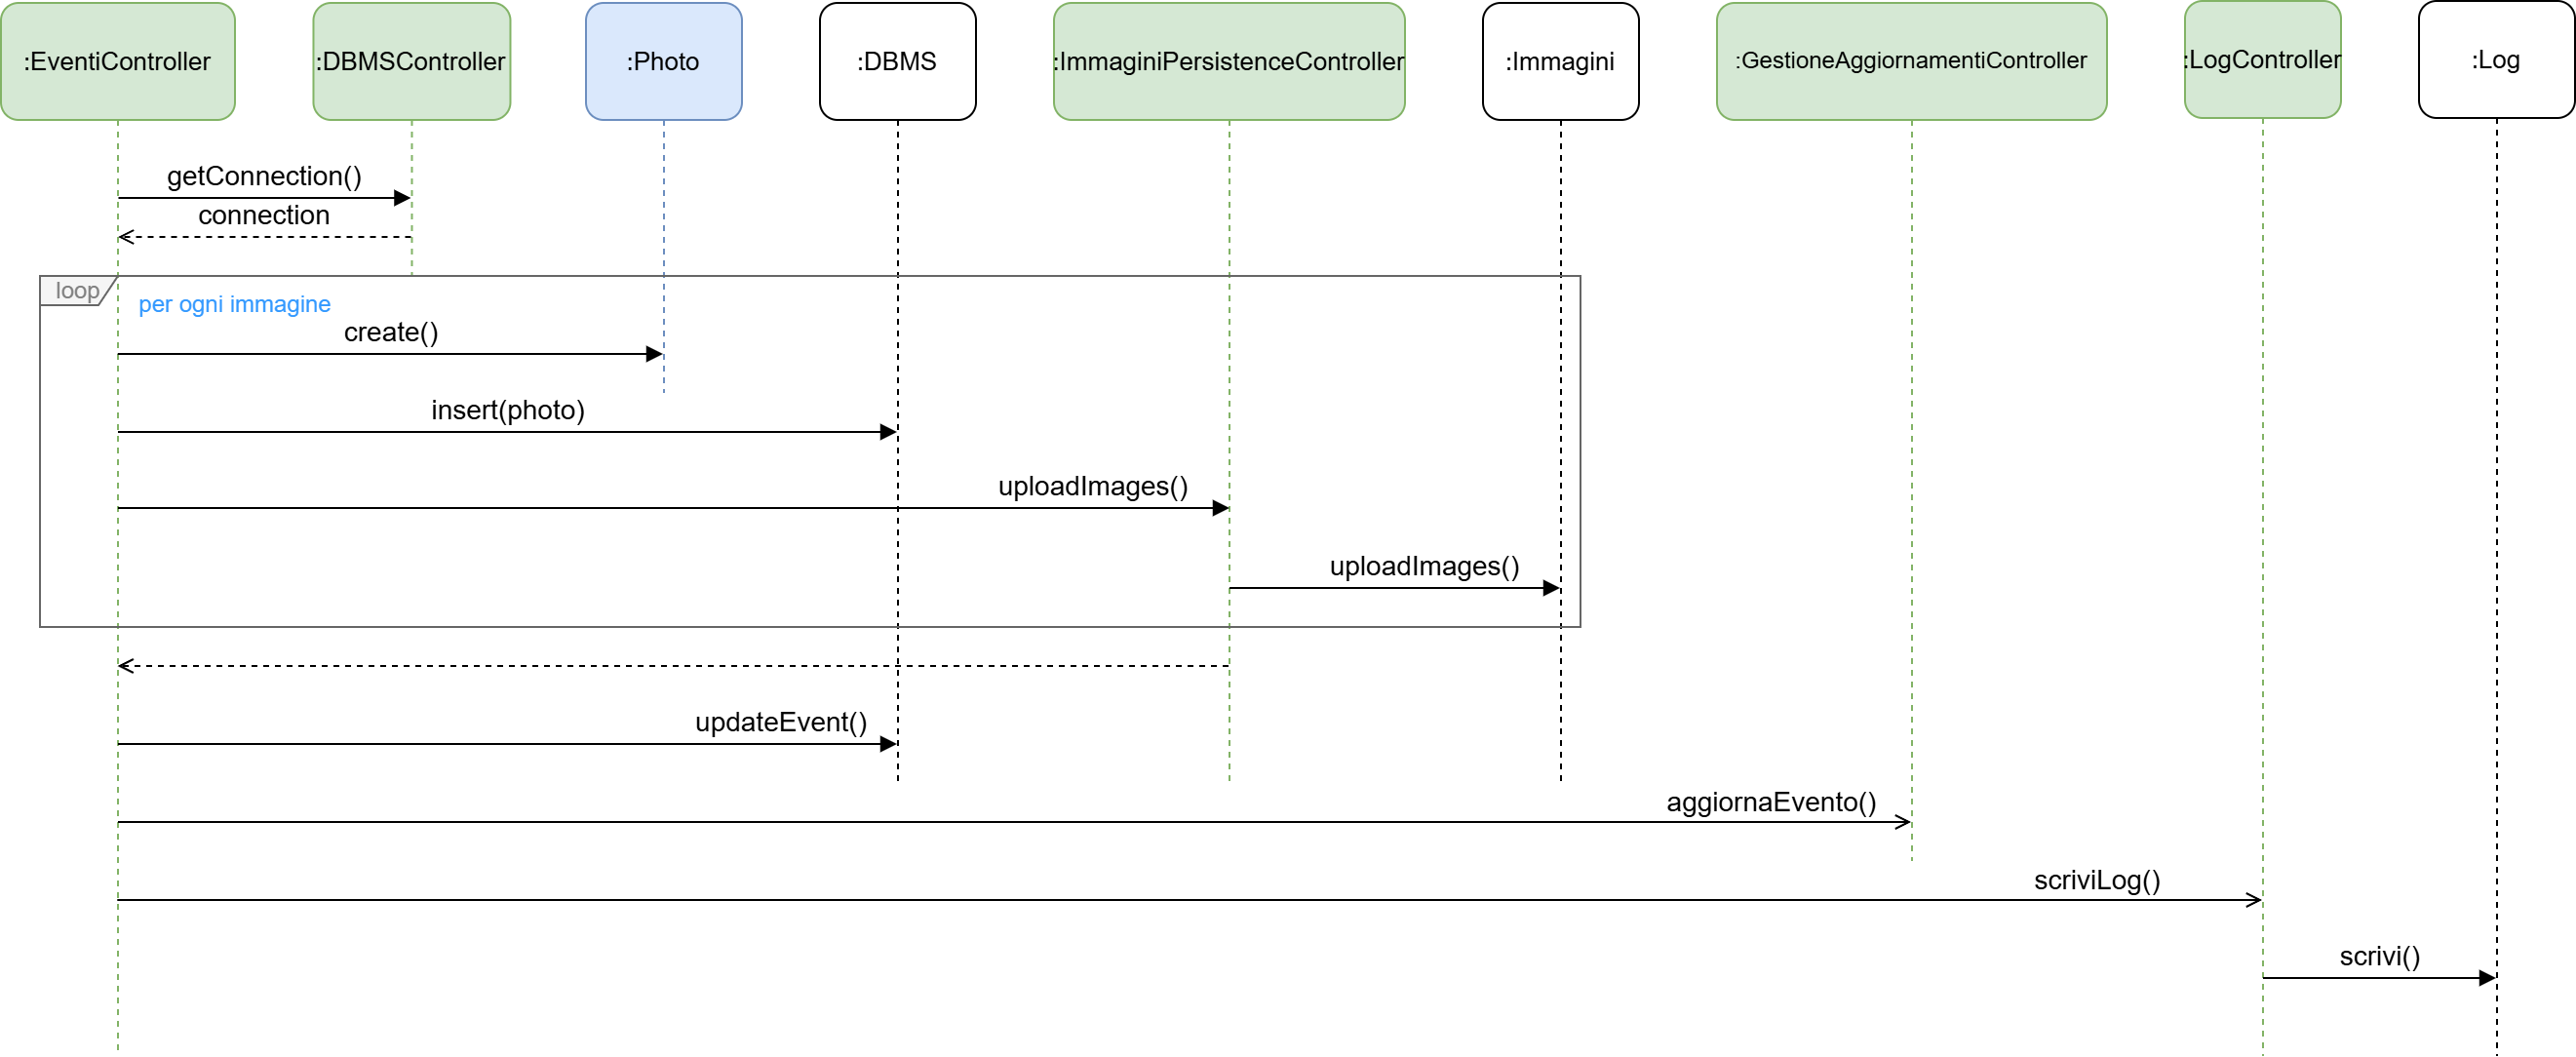
\includegraphics[width=\textwidth]{PIConfermaImmagini2.png}
    \caption{Interazione progettuale del server per il caricamento delle immagini }
\end{figure}	

L’accesso in lettura alle immagini però risulta così pubblico: la mancata definizione di ruoli comporta la carenza di controlli sull’autorizzazione delle richieste. Il problema si considera però ampiamente mitigato grazie alla creazione di hash randomici sufficientemente lunghi a rendere minima la probabilità di collisione.  La fruizione alle immagini senza la conoscenza degli hash, che richiede numerosi tentativi casuali nella speranza di trovare una combinazione corretta, risulta così molto improbabile e, nel caso di un attacco andato a buon fine, non fornisce ulteriori informazioni sul resto delle immagini.



\clearpage

\subsubsection{ Concorrenza }

Il caricamento delle immagini dalle Azure Functions al Container relativo all’evento è un’operazione lunga, soprattutto rispetto a tutte le altre eventualità. Il collegamento del server con il database relazionale comporta scelte di dominio e di sviluppo volte a permettere un uso ottimale delle sue connessioni, per ridurre al minimo il tempo di blocco delle risorse.

Per poter inviare i dati è necessario essere a conoscenza dell’hash dell’elemento Photo che andrà a corrispondere al file. L’hash viene generato nel momento della creazione dell’oggetto. Il suo salvataggio in memoria è bene che avvenga però solo a seguito dell’avvenuto caricamento del file multimediale, per evitare inutili scritture e cancellazioni sul database. Il momento della creazione di Photo è necessario che sia perciò distinto dal momento del suo salvataggio.

EF Core, per realizzare un’astrazione ad alto livello della relazione con il database, fornisce una rappresentazione logica degli elementi, mantenendo un collegamento con il loro corrispettivo fisico. Permette quindi di creare un oggetto subito e di  memorizzarlo in un secondo momento. 

La relazione uno a molti tra gli eventi e le immagini viene mappata fisicamente sugli oggetti Photo, salvando l’identificativo dell’Event associato. Nel momento del salvataggio verrà così modificata solo la tabella relativa a Photo. Tuttavia, il momento del suo salvataggio richiede il blocco in scrittura anche dell’Event interessato. L’oggetto Event risulta infatti coinvolto da un punto di vista logico, come si evince anche dalla presenza tra i suoi attributi virtuali(ovvero descritti dall’incrocio di dati da altre fonti) della lista delle immagini.

La parallelizzazione della trasmissione dei file multimediali al Container permette la minimizzazione del tempo necessario per lo svolgimento della richiesta. L’aggiunta dell’oggetto Photo al termine di ogni caricamento porterebbe al rischio di conflitti sullo stesso Event e il sovraccarico del database. Verranno quindi conservati temporaneamente gli oggetti logici Photo delle trasmissioni avvenute con successo, per salvarli poi in un’unico momento.

L’inserimento di tutti gli elementi Photo validi nella stessa transazione comporta  l'ottimizzazione dell’impatto sul database, riducendo i tempi di blocco sull’Event e quindi minimizzando le possibilità di collisione tra le richieste coinvolte.

\begin{figure}[h!]
    \centering
    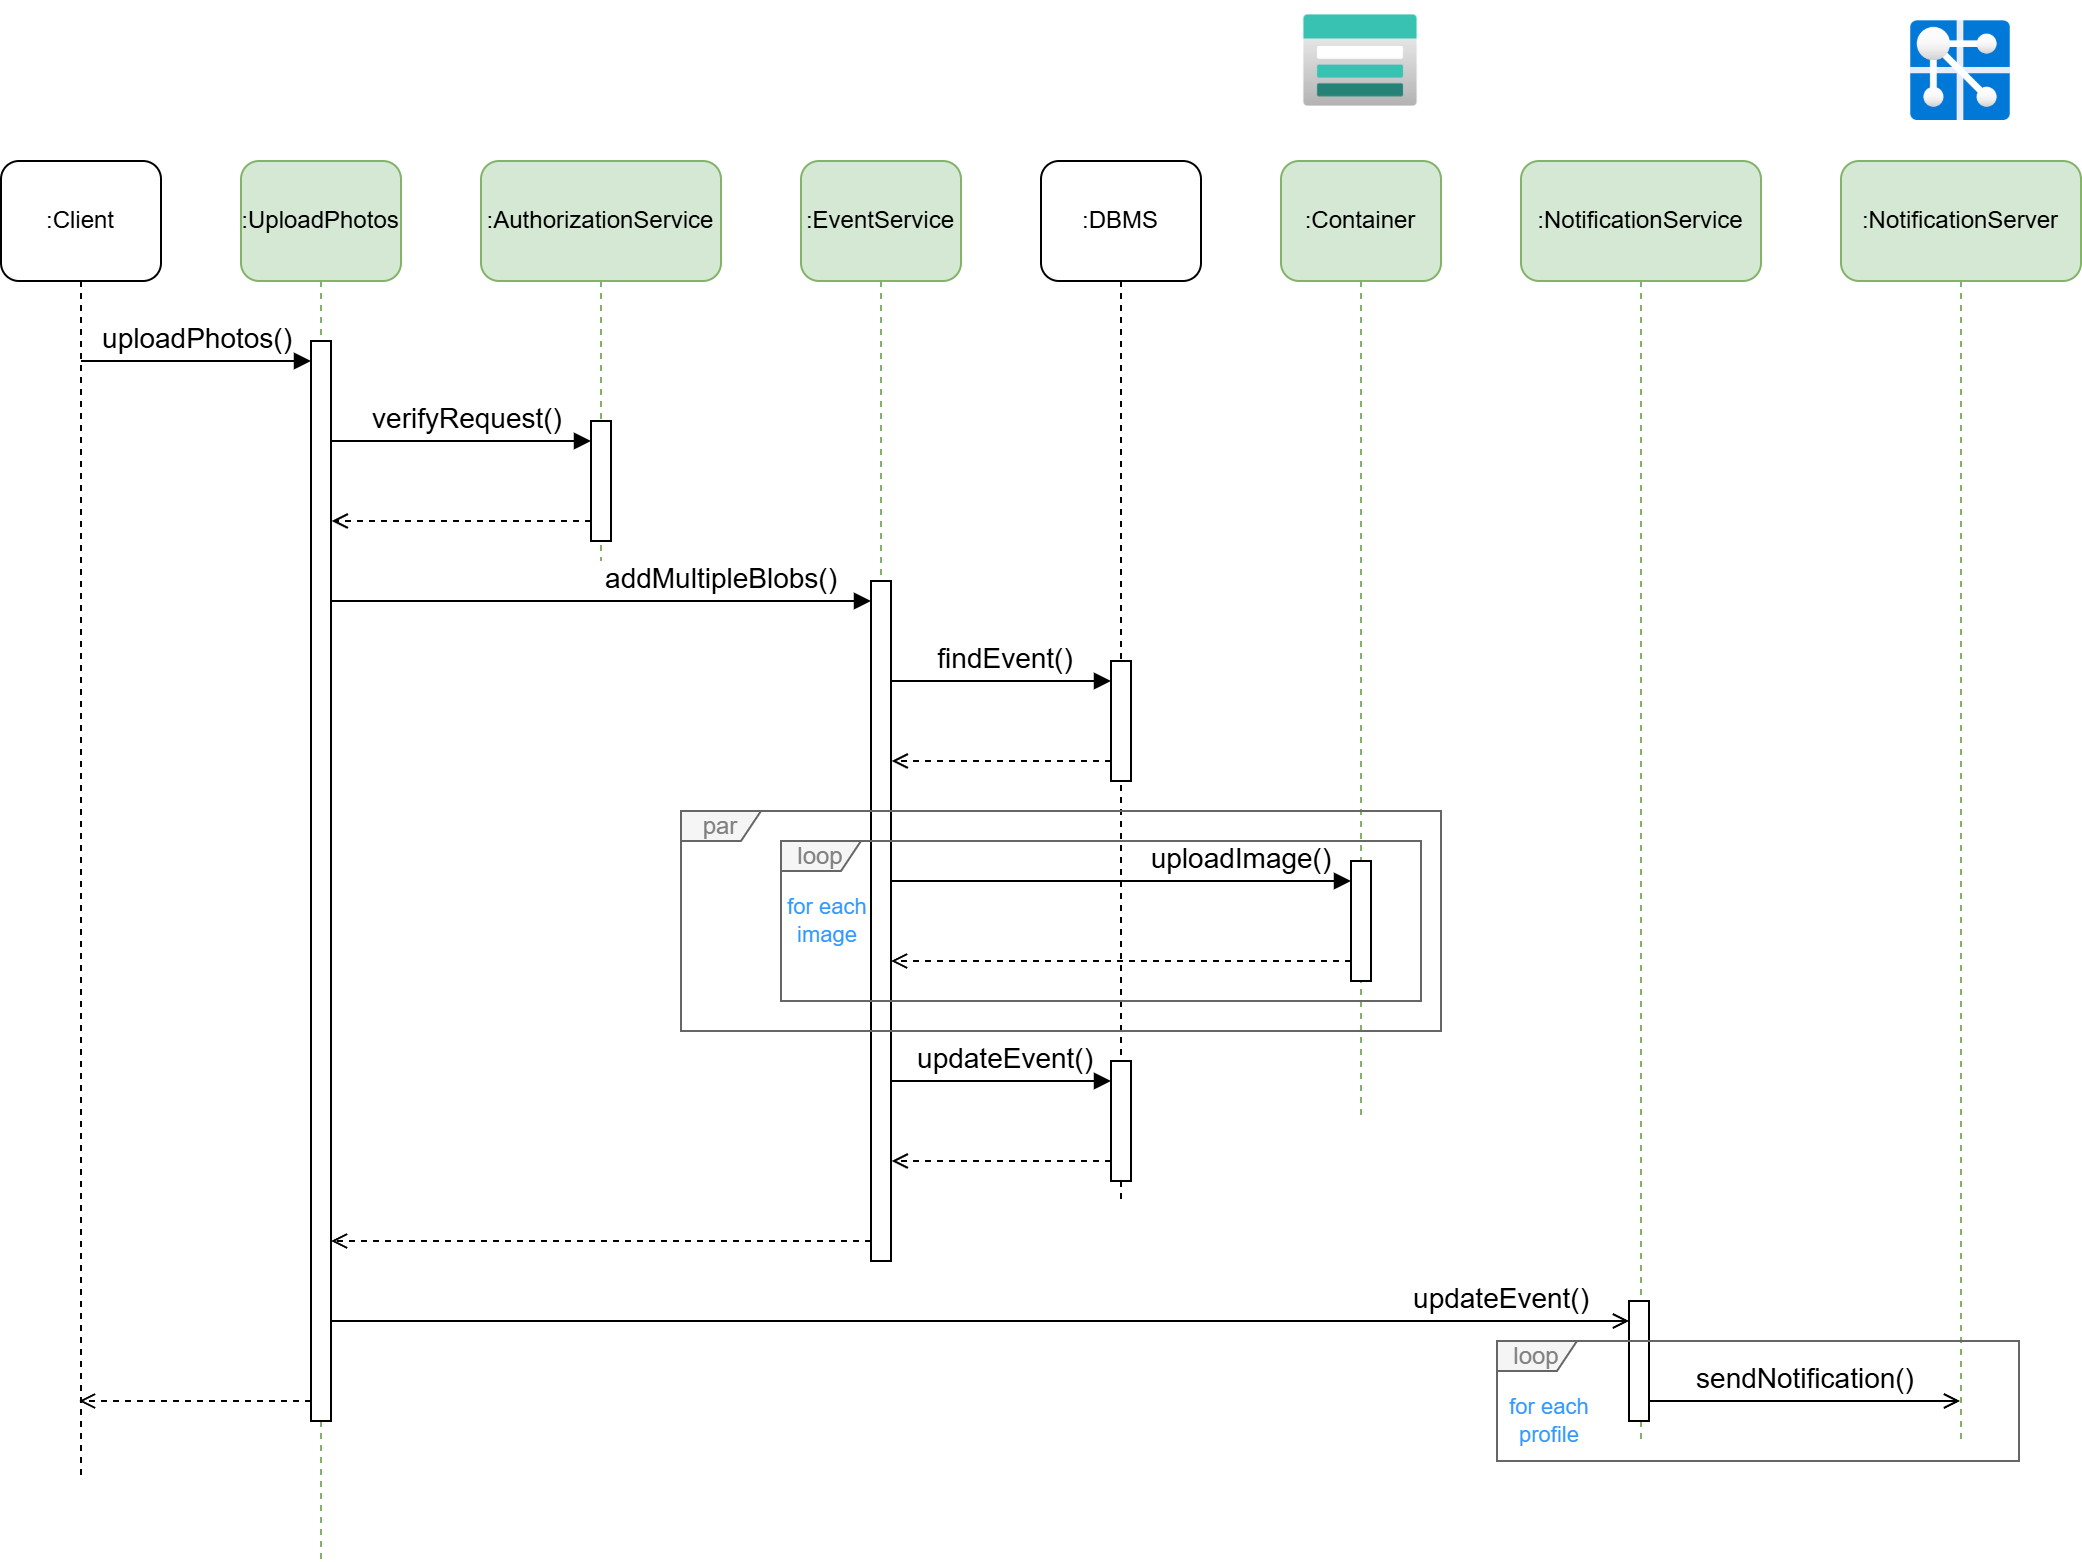
\includegraphics[width=\textwidth]{IICaricaImmagini.png}
    \caption{Interazione logica del server per il caricamento delle immagini }
\end{figure}

\clearpage

\chapter{Risultati}

\section{Velocità in lettura}

\begin{figure}[htbp]
    \begin{center}
        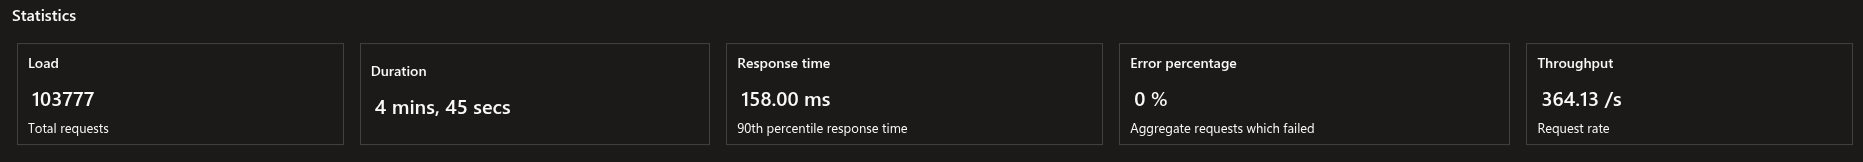
\includegraphics[width=\textwidth]{TestLettura1.png}
        \caption{158 ms su una media di 364 richieste al secondo}
    \end{center}
\end{figure}

\begin{figure}[htbp]
    \begin{center}
        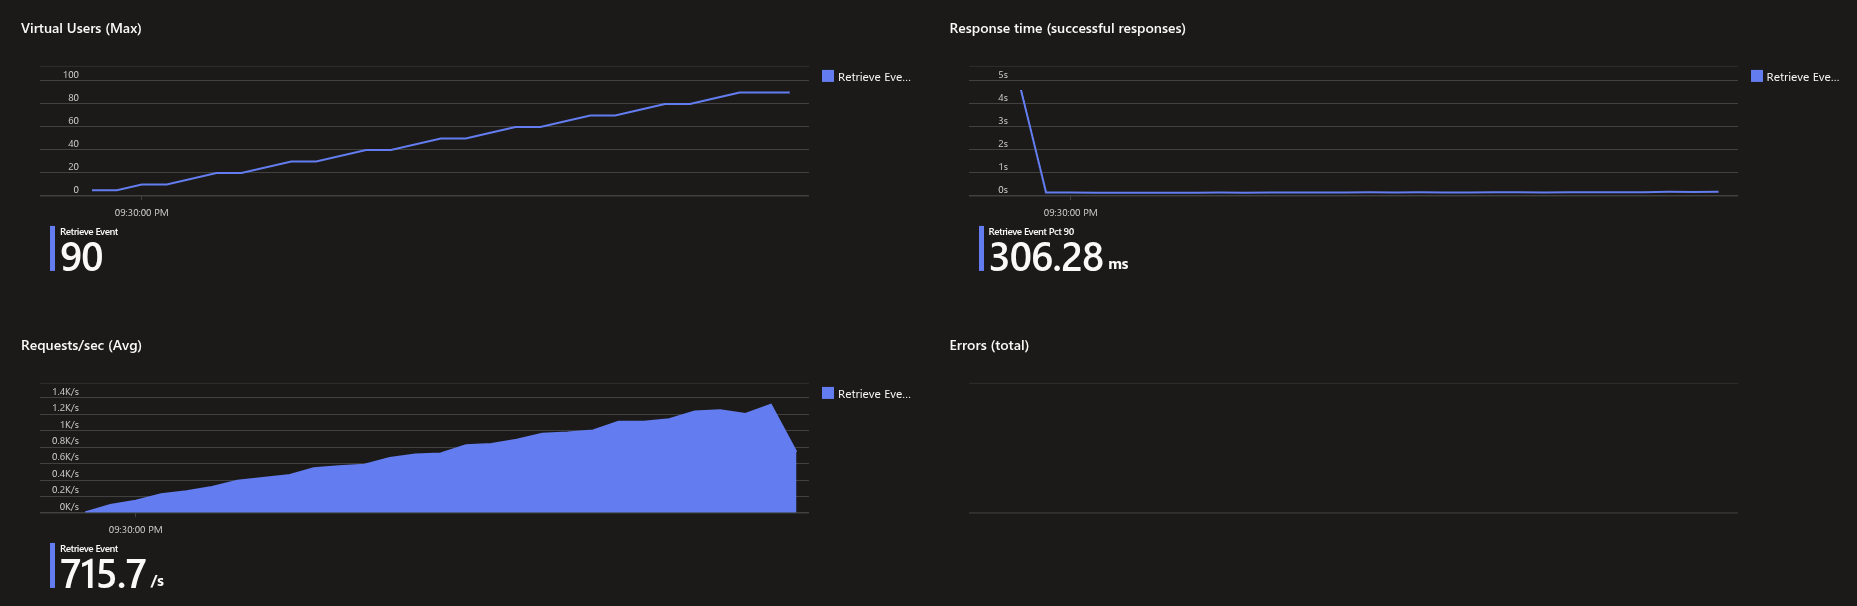
\includegraphics[width=\textwidth]{TestLettura2.png}
        \caption{il tempo di risposta non varia in base al numero di richieste}
    \end{center}
\end{figure}

\begin{figure}[htbp]
    \begin{center}
        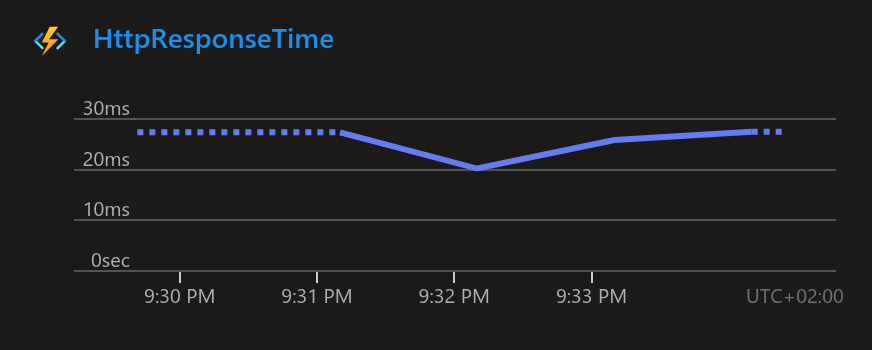
\includegraphics[width=\textwidth]{TestLettura3.png}
        \caption{Dettaglio della velocità senza tempo di trasmissione}
    \end{center}
\end{figure}
\clearpage
\section{Caricamento di immagini concorrenti}

\begin{figure}[htbp]
    \begin{center}
        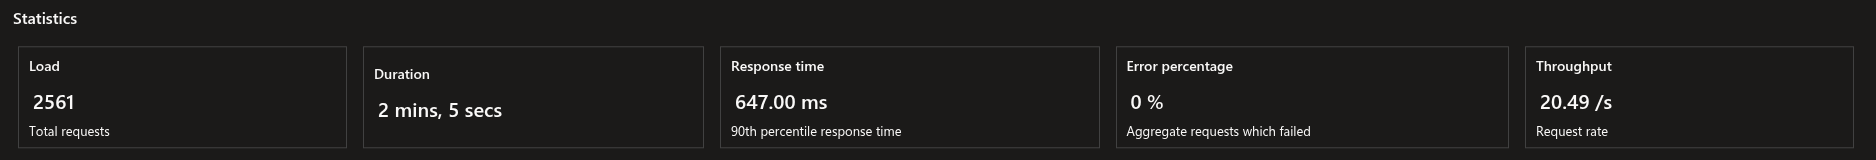
\includegraphics[width=\textwidth]{UploadImages1.png}
        \caption{2 MB di immagini in 600 ms 20 volte al secondo}  
    \end{center}
\end{figure}

\begin{figure}[htbp]
    \begin{center}
        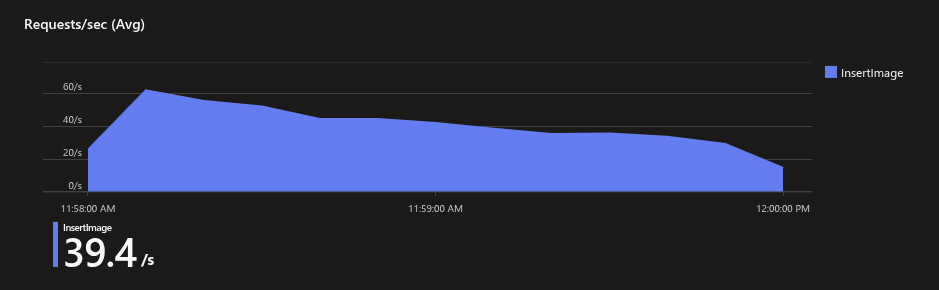
\includegraphics[width=\textwidth]{UploadImages3.png}
        \caption{Andamento delle richieste}  
    \end{center}
\end{figure}

\begin{figure}[htbp]
    \begin{center}
        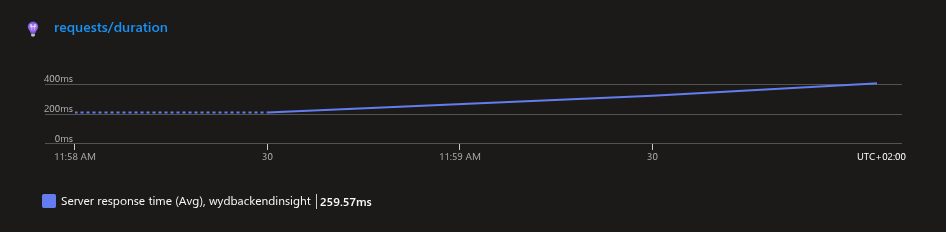
\includegraphics[width=\textwidth]{UploadImages2.png}
        \caption{Dettaglio della velocità richiesta dal server}
    \end{center}
\end{figure}


\clearpage
\chapter*{Conclusione}
\addcontentsline{toc}{chapter}{Conclusione}

\begin{figure}[htbp]
    \begin{center}
        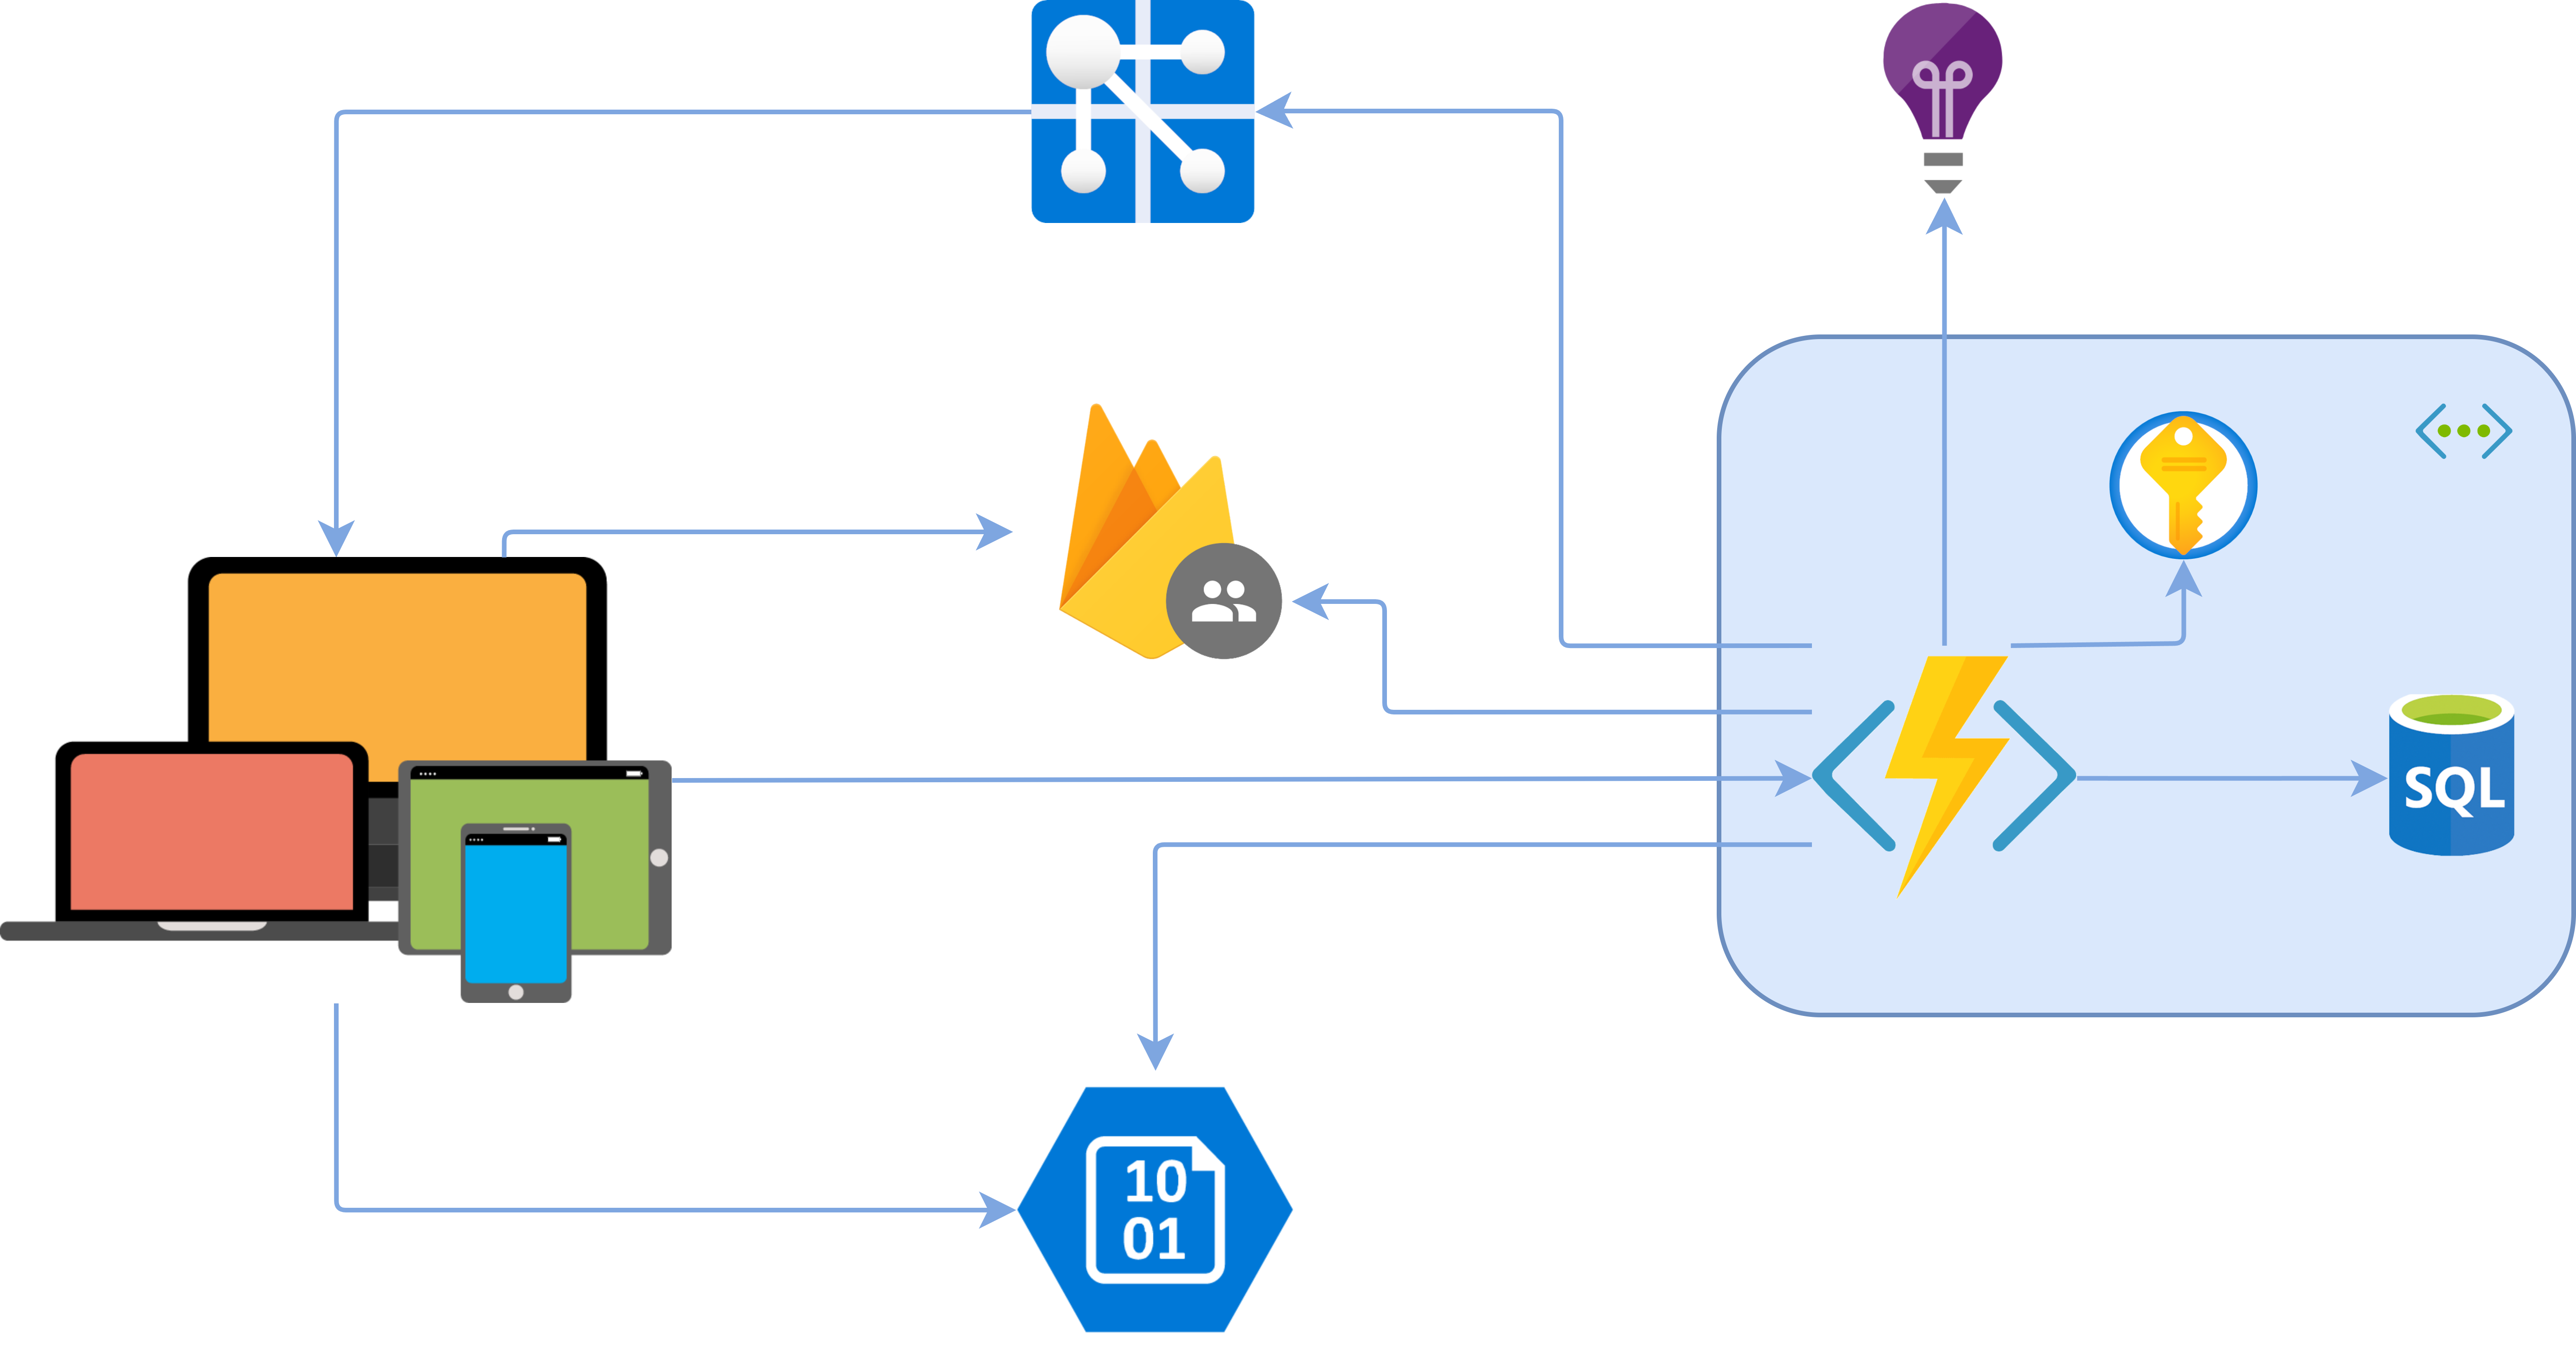
\includegraphics[width=\textwidth]{ImplementazioneArchitettura.png}
        \caption{Grafico dell'architettura finale}
    \end{center}
\end{figure}
\clearpage

\section{Sviluppi futuri}
Gli sviluppi futuri potranno comprendere, in base a decisioni di marketing:
\begin{itemize}
    \item La visualizzazione degli impegni degli altri profili
    \item L'implementazione di una chat per ogni gruppo
    \item Sviluppo di strumenti utili all'organizzazione dei gruppi, quali:
          \begin{itemize}
              \item form per combinare le disponibilità reciproche
              \item appunti condivisi(liste della spesa o note su chi porta cosa)
              \item calcolo delle spese compiute da ciascun componente
          \end{itemize}
    \item La creazione di profili pubblici che possono essere seguiti
    \item La creazione di eventi pubblici
    \item Una funzionalità di ricerca degli eventi o dei profili pubblici
    \item Supporto alla gestione di prenotazione e organizzazione degli eventi, dalle liste di attesa alla vendita dei biglietti
    \item La possibilità per le aziende di gestire in locale il proprio server e i relativi dati
\end{itemize}
\clearpage

\chapter*{Fonti bibliografiche e sitografia}
\addcontentsline{toc}{chapter}{Fonti bibliografiche e sitografia}

Object Management Group, OMG Unified Modelling Language Version 2.5.1, December 2017, https://www.omg.org/spec/UML/2.5.1/PDF

\end{document}requisiti